%==============================================================================
% tento soubor pouzijte jako zaklad
% this file should be used as a base for the thesis
% Autoři / Authors: 2008 Michal Bidlo, 2019 Jaroslav Dytrych
% Kontakt pro dotazy a připomínky: dytrych@fit.vutbr.cz
% Contact for questions and comments: dytrych@fit.vutbr.cz
%==============================================================================
% kodovani: UTF-8 (zmena prikazem iconv, recode nebo cstocs)
% encoding: UTF-8 (you can change it by command iconv, recode or cstocs)
%------------------------------------------------------------------------------
% zpracování / processing: make, make pdf, make clean
%==============================================================================
% Soubory, které je nutné upravit: / Files which have to be edited:
%   projekt-20-literatura-bibliography.bib - literatura / bibliography
%   projekt-01-kapitoly-chapters.tex - obsah práce / the thesis content
%   projekt-30-prilohy-appendices.tex - přílohy / appendices
%==============================================================================
\documentclass[]{fitthesis} % bez zadání - pro začátek práce, aby nebyl problém s překladem
%\documentclass[english]{fitthesis} % without assignment - for the work start to avoid compilation problem
%\documentclass[zadani]{fitthesis} % odevzdani do wisu a/nebo tisk s barevnými odkazy - odkazy jsou barevné
%\documentclass[english,zadani]{fitthesis} % for submission to the IS FIT and/or print with color links - links are color
%\documentclass[zadani,print]{fitthesis} % pro černobílý tisk - odkazy jsou černé
%\documentclass[english,zadani,print]{fitthesis} % for the black and white print - links are black
%\documentclass[zadani,cprint]{fitthesis} % pro barevný tisk - odkazy jsou černé, znak VUT barevný
%\documentclass[english,zadani,cprint]{fitthesis} % for the print - links are black, logo is color
% * Je-li práce psaná v anglickém jazyce, je zapotřebí u třídy použít 
%   parametr english následovně:
%   If thesis is written in english, it is necessary to use 
%   parameter english as follows:
%      \documentclass[english]{fitthesis}
% * Je-li práce psaná ve slovenském jazyce, je zapotřebí u třídy použít 
%   parametr slovak následovně:
%   If the work is written in the Slovak language, it is necessary 
%   to use parameter slovak as follows:
%      \documentclass[slovak]{fitthesis}
% * Je-li práce psaná v anglickém jazyce se slovenským abstraktem apod., 
%   je zapotřebí u třídy použít parametry english a enslovak následovně:
%   If the work is written in English with the Slovak abstract, etc., 
%   it is necessary to use parameters english and enslovak as follows:
%      \documentclass[english,enslovak]{fitthesis}

% Základní balíčky jsou dole v souboru šablony fitthesis.cls
% Basic packages are at the bottom of template file fitthesis.cls
% zde můžeme vložit vlastní balíčky / you can place own packages here
\usepackage{amsmath}
\usepackage{algorithm}
\usepackage[noend]{algpseudocode}

\newcommand{\sfunction}[1]{\textsf{\textsc{#1}}}
\algrenewcommand\algorithmicforall{\textbf{foreach}}
\algrenewcommand\algorithmicindent{.8em}
% Kompilace po částech (rychlejší, ale v náhledu nemusí být vše aktuální)
% Compilation piecewise (faster, but not all parts in preview will be up-to-date)
% \usepackage{subfiles}

% Nastavení cesty k obrázkům
% Setting of a path to the pictures
%\graphicspath{{obrazky-figures/}{./obrazky-figures/}}
%\graphicspath{{obrazky-figures/}{../obrazky-figures/}}

%---rm---------------
\renewcommand{\rmdefault}{lmr}%zavede Latin Modern Roman jako rm / set Latin Modern Roman as rm
%---sf---------------
\renewcommand{\sfdefault}{qhv}%zavede TeX Gyre Heros jako sf
%---tt------------
\renewcommand{\ttdefault}{lmtt}% zavede Latin Modern tt jako tt

% vypne funkci šablony, která automaticky nahrazuje uvozovky,
% aby nebyly prováděny nevhodné náhrady v popisech API apod.
% disables function of the template which replaces quotation marks
% to avoid unnecessary replacements in the API descriptions etc.
\csdoublequotesoff

% =======================================================================
% balíček "hyperref" vytváří klikací odkazy v pdf, pokud tedy použijeme pdflatex
% problém je, že balíček hyperref musí být uveden jako poslední, takže nemůže
% být v šabloně
% "hyperref" package create clickable links in pdf if you are using pdflatex.
% Problem is that this package have to be introduced as the last one so it 
% can not be placed in the template file.
\ifWis
\ifx\pdfoutput\undefined % nejedeme pod pdflatexem / we are not using pdflatex
\else
  \usepackage{color}
  \usepackage[unicode,colorlinks,hyperindex,plainpages=false,pdftex]{hyperref}
  \definecolor{hrcolor-ref}{RGB}{223,52,30}
  \definecolor{hrcolor-cite}{HTML}{2F8F00}
  \definecolor{hrcolor-urls}{HTML}{092EAB}
  \hypersetup{
	linkcolor=hrcolor-ref,
	citecolor=hrcolor-cite,
	filecolor=magenta,
	urlcolor=hrcolor-urls
  }
  \def\pdfBorderAttrs{/Border [0 0 0] }  % bez okrajů kolem odkazů / without margins around links
  \pdfcompresslevel=9
\fi
\else % pro tisk budou odkazy, na které se dá klikat, černé / for the print clickable links will be black
\ifx\pdfoutput\undefined % nejedeme pod pdflatexem / we are not using pdflatex
\else
  \usepackage{color}
  \usepackage[unicode,colorlinks,hyperindex,plainpages=false,pdftex,urlcolor=black,linkcolor=black,citecolor=black]{hyperref}
  \definecolor{links}{rgb}{0,0,0}
  \definecolor{anchors}{rgb}{0,0,0}
  \def\AnchorColor{anchors}
  \def\LinkColor{links}
  \def\pdfBorderAttrs{/Border [0 0 0] } % bez okrajů kolem odkazů / without margins around links
  \pdfcompresslevel=9
\fi
\fi
% Řešení problému, kdy klikací odkazy na obrázky vedou za obrázek
% This solves the problems with links which leads after the picture
\usepackage[all]{hypcap}

\usepackage{pythonhighlight}

\lstset{numbers=left,
firstnumber=1,
numberfirstline=true,
escapeinside={(*}{*)}}

\usepackage{dirtree}

\usepackage[figuresleft]{rotating}
\usepackage{pdflscape}

% Informace o práci/projektu / Information about the thesis
%---------------------------------------------------------------------------
\projectinfo{
  %Prace / Thesis
  project={BP},            %typ práce BP/SP/DP/DT/DR  / thesis type (SP = term project)
  year={2019},             % rok odevzdání / year of submission
  date=\today,             % datum odevzdání / submission date
  %Nazev prace / thesis title
  title.cs={Interpret vysokoúrovňových Petriho sítí v Pythonu},  % název práce v češtině či slovenštině (dle zadání) / thesis title in czech language (according to assignment)
  title.en={High-Level Petri Nets Interpreter in Pyhon}, % název práce v angličtině / thesis title in english
  %title.length={14.5cm}, % nastavení délky bloku s titulkem pro úpravu zalomení řádku (lze definovat zde nebo níže) / setting the length of a block with a thesis title for adjusting a line break (can be defined here or below)
  %Autor / Author
  author.name={Danil},   % jméno autora / author name
  author.surname={Grigorev},   % příjmení autora / author surname 
  %author.title.p={Bc.}, % titul před jménem (nepovinné) / title before the name (optional)
  %author.title.a={Ph.D.}, % titul za jménem (nepovinné) / title after the name (optional)
  %Ustav / Department
  department={UITS}, % doplňte příslušnou zkratku dle ústavu na zadání: UPSY/UIFS/UITS/UPGM / fill in appropriate abbreviation of the department according to assignment: UPSY/UIFS/UITS/UPGM
  % Školitel / supervisor
  %, doc. Ing., Ph.D.
  supervisor.name={Vladimír},   % jméno školitele / supervisor name 
  supervisor.surname={Janoušek},   % příjmení školitele / supervisor surname
  supervisor.title.p={doc. Ing.},   %titul před jménem (nepovinné) / title before the name (optional)
  supervisor.title.a={Ph.D.},    %titul za jménem (nepovinné) / title after the name (optional)
  % Klíčová slova / keywords
  keywords.cs={Petriho síť, Python, HLPN, simulace, simulator, topení, interpret, real-time, SNAKES, graf}, % klíčová slova v českém či slovenském jazyce / keywords in czech or slovak language
  keywords.en={Petri Net, Python, HLPN, simulation, interpret, real-time, SNAKES, graph}, % klíčová slova v anglickém jazyce / keywords in english
  %keywords.en={Here, individual keywords separated by commas will be written in English.},
  % Abstrakt / Abstract
  abstract.cs={Tato práce je zaměřená na implementací interpretu vysokoúrovňových Petriho sítí v jayzce Python za použítí knihovny SNAKES. Je schopná provadění a pokročilé vizualizace navyřených sítí, které jsou popsané v jayzce Python. Vysledný simulator odpovidá zasadům distribuovaného systému, a podporuje provádí v realném čase. Konečný užívatel bude mít příležitost vyzkoušet intuitivní API pro vytvoření a spouštění vysokoúrovňových Petriho sítí.}, % abstrakt v českém či slovenském jazyce / abstract in czech or slovak language
  abstract.en={This work is targeting a goal of implementing a high level Petri net interpret in Python. The implementation is based on SNAKES library. The final product is capable of executing and visualising Petri nets, created by user. The simulator is based on distributed systems theory and is executed in real-time. The end user is able to experience a simple and human-friendly API, made for creation and execution of High-Level Petri Nets.}, % abstrakt v anglickém jazyce / abstract in english
  %abstract.en={An abstract of the work in English will be written in this paragraph.},
  % Prohlášení (u anglicky psané práce anglicky, u slovensky psané práce slovensky) / Declaration (for thesis in english should be in english)
  declaration={Prohlašuji, že jsem tuto bakalářskou práci vypracoval samostatně pod vedením pana Janoušeka Vladimíra, doc. Ing., Ph.D.
Uvedl jsem všechny literární prameny a publikace, ze kterých jsem čerpal.},
  %declaration={I declare that I have prepared this Bachelor´s/Master´s/dissertation thesis independently, under the supervision of ...
% ... provided me with further information.
% I listed all of the literary sources and publications that I have used.},
  % Poděkování (nepovinné, nejlépe v jazyce práce) / Acknowledgement (optional, ideally in the language of the thesis)
  acknowledgment={Děkuji Doc. Ing. Vladimíru Janouškovi za obrovskou pomoc a poradu pří psání této bakalářské práce.},
  %acknowledgment={Here it is possible to express thanks to the supervisor and to the people which provided professional help
%(external submitter, consultant, etc.).},
  % Rozšířený abstrakt (cca 3 normostrany) - lze definovat zde nebo níže / Extended abstract (approximately 3 standard pages) - can be defined here or below
  %extendedabstract={Do tohoto odstavce bude zapsán rozšířený výtah (abstrakt) práce v českém (slovenském) jazyce.},
  %faculty={FIT}, % FIT/FEKT/FSI/FA/FCH/FP/FAST/FAVU/USI/DEF
  faculty.cs={Fakulta informačních technologií}, % Fakulta v češtině - pro využití této položky výše zvolte fakultu DEF / Faculty in Czech - for use of this entry select DEF above
  faculty.en={Faculty of Information Technology}, % Fakulta v angličtině - pro využití této položky výše zvolte fakultu DEF / Faculty in English - for use of this entry select DEF above
  department.cs={Ústav matematiky}, % Ústav v češtině - pro využití této položky výše zvolte ústav DEF nebo jej zakomentujte / Department in Czech - for use of this entry select DEF above or comment it out
  department.en={Institute of Mathematics} % Ústav v angličtině - pro využití této položky výše zvolte ústav DEF nebo jej zakomentujte / Department in English - for use of this entry select DEF above or comment it out
}

% Rozšířený abstrakt (cca 3 normostrany) - lze definovat zde nebo výše / Extended abstract (approximately 3 standard pages) - can be defined here or above
%\extendedabstract{Do tohoto odstavce bude zapsán výtah (abstrakt) práce v českém (slovenském) jazyce.}

% nastavení délky bloku s titulkem pro úpravu zalomení řádku - lze definovat zde nebo výše / setting the length of a block with a thesis title for adjusting a line break - can be defined here or above
%\titlelength{14.5cm}


% řeší první/poslední řádek odstavce na předchozí/následující stránce
% solves first/last row of the paragraph on the previous/next page
\clubpenalty=10000
\widowpenalty=10000

% checklist
\newlist{checklist}{itemize}{1}
\setlist[checklist]{label=$\square$}

\setlength{\parskip}{0pt}

\begin{document}
  % Vysazeni titulnich stran / Typesetting of the title pages
  % ----------------------------------------------
  \maketitle
  % Obsah
  % ----------------------------------------------
  {\hypersetup{hidelinks}\tableofcontents}
  
  % Seznam obrazku a tabulek (pokud prace obsahuje velke mnozstvi obrazku, tak se to hodi)
  % List of figures and list of tables (if the thesis contains a lot of pictures, it is good)
  \ifczech
    \renewcommand\listfigurename{Seznam obrázků}
  \fi
  \ifslovak
    \renewcommand\listfigurename{Zoznam obrázkov}
  \fi
  % \listoffigures
  
  \ifczech
    \renewcommand\listtablename{Seznam tabulek}
  \fi
  \ifslovak
    \renewcommand\listtablename{Zoznam tabuliek}
  \fi
  % \listoftables 

  \ifODSAZ
    \setlength{\parskip}{0.5\bigskipamount}
  \else
    \setlength{\parskip}{0pt}
  \fi

  % vynechani stranky v oboustrannem rezimu
  % Skip the page in the two-sided mode
  \iftwoside
    \cleardoublepage
  \fi

  % Text prace / Thesis text
  % ----------------------------------------------
  \chapter{Úvod}
\label{chap:uvod}

Formalizmus Petriho sítí v~současné době nemá tolik uznání, kolík si tento modelovací prostředek zaslouží. Cílem této bakalářské práce je ukázat čtenáři, kde všude se dá uplatnit matematický model Petriho sítí, a jaké výhody to přináší. Tato práce je zaměřena na docela populární téma distribuovaných systému, o~kterých byste se po přečtení mohli dozvědět více.

Ve výsledku byste pochopili princip práce simulátoru v~reálném čase, založeném na využití modelovacích technik Petriho sítí za použití knihovny SNAKES, který má předpoklady pro využití v~distribuovaných systémech. Vzhledem k~tomu, že takový systém je hodně závislý na komunikací se svými vzdálenými prvky, tak se v~průběhu vysvětlí principy protokolu MQTT, který se stal základem implementace simulátoru a jeho komunikačních kanálů. Nakonec byste byli schopni odzkoušet simulátor v~praxi, a podívat se podrobně na Petriho sítě, navržené pro ukázkovou aplikaci. Tato aplikace bude vytvořena pro demonstrační účely a založena na teorii distribuovaných systémů.

Výsledný simulační nástroj bude vytvořený tak, abyste mohli snadno získat představu o~současném stavu implementací nebo běhu simulace, za využití uživatelsky zaměřeného vizualizačního modulu knihovny SNAKES. Generované obrázky tohoto modulu sestaví nemalou část obsahu této práce. Díky naimplementovaným rozšířením bude čtenář schopný snadno vytvořit sadu pro svůj model.

Vzhledem k~existenci hotového nástroje pro modelování a simulaci, bude část této práce věnovaná popisu vytvoření aplikace za účelem usnadnění procesu modelování a seznámení čtenáře s~hotovým produktem a postupem pro jeho nastavení.

\chapter{Přehled teorie}
\label{chapp:prehled}

V~této kapitole jsou popsané teoretické základy Petriho sítí. Taky tato kapitola se soustředí na popis několika podtříd Petriho sítě, zejména na \uv{Vysokoúrovňové Petriho sítě} \ref{subsec:hlpn} a \uv{Značkované Petriho Sítě} \ref{subsec:marked-pn} a  včetně přehledu míst, kde se tento modelovací prostředek používá, a hraje významnou roli \ref{sec:pn-application}.

Dalším účelem této kapitoly je seznámení čtenáře s~matematickými popisy Petriho síti (\ref{subsec:marked-pn}, \ref{subsec:hlpn}) a grafy Petriho sítí \ref{subsec:hlpn-graph}, které jsou nezbytné pro porozumění principu prace simulátoru \ref{sec:sim-theory}.

Do obsahu patří popis protokolu MQTT \ref{subsec:mqtt-proto}, na kterém je založena externí komunikace simulátoru \ref{sec:mqtt_impl}.

Taky se tady zmíním o~simulační teorii, zaměřené na simulaci Petriho síti v~reálném čase. Vyjasní se tím pojem distribuovaných systému \ref{subsec:distr_system}, HWIL \ref{subsec:hwil} a jejích vztah s~Petriho sítěmi.

\section{Petriho sítě}

V~současné době se Petriho sítě často používají jako modelovací prostředek pro modelování chování systému, za účelem pochopení jeho slabších stránek, ještě než se systém nasadí do provozu. Vyplňuje tím pádem mezeru mezi slovním popisem a návrhem (pomoci takových modelovacích prostředků jako \href{https://en.wikipedia.org/wiki/Unified_Modeling_Language}{UML}), a implementací. Použití Petriho síti pro účel modelování je velice vhodné, jen velmi málo modelovacích prostředku dokáže popsat ne jenom systém jako celek, ale i zjistit slabší stránky jeho implementace, ještě před implementační fází. Stejně tak platí i pro testovací fází -- některé chyby se dají objevit jenom po implementací, když Petriho sítě částečně řeší tento problém ještě ve fází návrhu.

\paragraph{Definice}

Petriho síť ($PN$) je čtyřce, $PN = \left(P, T, I, O\right)$ kde:
  \begin{itemize}
    \item $P = \left\{p_1, p_2, \cdots , p_n\right\}$ je konečná množina míst, $n >= 0$; \\
    \item $T = \left\{t_1, t_2, \cdots , t_m\right\}$ je konečná množina přechodů, $m >= 0$; \\
    \item $I = T \rightarrow P^\infty$ je vstupní funkce, propojující přechody s~množinou vstupních míst; \\
    \item $O = P \rightarrow T^\infty$ je výstupní funkce, propojující výstupní místa s~množinou přechodů; \\
  \end{itemize}
P $\vee$ T = $\varnothing$, P $\wedge$ T != $\varnothing$.

\section{Typy Petriho sítě}

V~této sekci budou popsané teoretické základy několika druhů Petriho sítí, značkovaných -- \ref{subsec:marked-pn} a Vysokoúrovňových Petriho sítí -- \ref{subsec:hlpn} a jejich grafu -- \ref{subsec:hlpn-graph} a jak se v~takovém grafu provádí přechod -- \ref{subsec:graph-transition}. Taky bude něco málo zmíněno o~Stochastických Petriho sítí -- \ref{subsec:timed-pn}.

\subsection{Značkované Petriho sítě}
\label{subsec:marked-pn}
Značkované Petriho sítě (ZPS) zavadí takový pojem jako značka nebo \uv{token}. Značka je základní prvek v~ZPS, umožnující její vykonávaní. Vykonávaní se provádí provedením přechodu, během kterého se vymaže odpovídající počet značek z~množiny vstupních míst, a do výstupních míst se potřebný počet značek vloží. Tato operace se může vykonávat, dokud nezbude žádný povolený přechod. Na této myšlence je založena simulace provádění Petriho sítě.

Přechod v~PS je povolen, dokud každé ze vstupních míst propojených s~daným přechodem obsahuje alespoň jednu značku.

Pri vykonávaní sítě Petri vznikají dvě posloupnosti -- posloupnost značek a posloupnost přechodu, které byly provedeny. Tyto dvě posloupnosti popisuji zcela vykonání Petriho sítě. \cite[p.18--19]{PNandMoS}

Každá ze šipek v~Petriho sítí má váhu. Váha reprezentuje číslo tokenů, které se musí nacházet ve vstupním místě pro to, aby přechod byl proveditelný. Při provedení váha určuje, kolík tokenů se vyjme ze vstupního místa, nebo kolík se jích vloží do místa výstupního.

\paragraph{Definice}

Značkovaná Petriho síť je šestice $PN = \left(P, T, I, O, W, M_0\right)$
\begin{itemize}
  \item $P = \left\{p_1, p_2, \cdots , p_n\right\}$ je konečná množina míst, $n >= 0$; \\
  \item $T = \left\{t_1, t_2, \cdots , t_m\right\}$ je konečná množina přechodů, $m >= 0$; \\
  \item $I = T \rightarrow P^\infty$ je vstupní funkce, propojující přechody s~množinou vstupních míst; \\
  \item $O = P \rightarrow T^\infty$ je výstupní funkce, propojující výstupní místa s~množinou přechodů; \\
  \item $W = F \rightarrow \left\{1, 2, 3, \cdots \right\}$ je váhová funkce; \\
  \item $M_0$ je multimnožina počátečních značek;
\end{itemize}
P $\vee$ T = $\varnothing$, P $\wedge$ T != $\varnothing$.

Díky možnosti vykonávat Petriho síť vzniká příležitost, vytvořit simulační nastroj, který je založen na zmíněných teoretických základech. Podrobný popis simulátoru viz. \ref{chap:implementation}.

\subsection{Stochastické Petriho sítě}
\label{subsec:timed-pn}

Podtřída Stochastických Petriho sítí [Stochastic Petri Net] rozšiřuje pojem značkovaných Petriho sítí o~jednu důležitou zásadu -- přechod může být označen časovou funkcí. Aby se takový přechod provedl, ten čas musí uplynout, až potom se vyjmou tokeny ze vstupních míst a vloží se do výstupních. Časová funkce nemusí být konstantní, může být závislá na stochastickém procesu, ale v~rámci této práce se použilo jenom konstantní čekání na přechod, jelikož chování simulátoru musí být deterministické. Více o~implementačních detailech viz. \ref{subsec:timed_pl}.

\subsection{Vysokoúrovňové Petriho sítě}
\label{subsec:hlpn}

Vysokoúrovňové Petriho sítě (High Level Petri Nets) jsou dalším rozšířením Petriho sítí, které umožňují jednodušší modelování takových procesů, pro které jsou důležité výpočty a matematické výrazy. Celkově je tento druh Petriho sítě pohodlnější pro modelování toku řízení kódu nějakého programu a ve své podstatě připomíná grafické programování.

\paragraph{Definice} \cite[p.11--12]{pnstd54}

High Level Petri Net (HLPN) je struktura $HLPN = \left( P; T; D; T_{ype}; P_{re}; P_{ost}; M_0\right) $ kde:

\begin{itemize}
  \item $P$ je konečná množina míst. \\
  \item $T$ je konečná množina přechodu, pro kterou platí $\left(P \cup T = \varnothing\right)$. \\
  \item $D$ je konečná neprázdná množina domén, kde každý element domény se jmenuje typ. \\
  \item $T_{ype}$ : $P \cap T \rightarrow D$ je funkce pro přidání typu do míst a určeni typu přechodu.
  \item $P_{re}$, $P_{ost}$ : $TRANS$ $\rightarrow$ $\mu PLACE$ jsou pre a post kondici pro které platí: \\
  \begin{center}
    \item $TRANS$ = $\left\{\left(t, m\right)\:\vert\:t \in T, m \in T_{ype} \left( t \right)\right\}$ \\
    \item $PLACE$ = $\left\{\left(p, g\right)\:\vert\:p \in P, g \in T_{ype} \left( p \right)\right\}$ \\
  \end{center}
  \item $M_0$ je $\mu PLACE$ je multimnožina počátečních značek.
\end{itemize}

\subsection{Pravidlo pro provedení přechodu}
\label{subsec:graph-transition}

Pokud je dané, že konečná multimnožina $T_\mu$ je zapnuta pro značku $M$, tedy přechod v~$HLPN$ muže byt proveden pro značku $M'$ následujícím způsobem \cite[p.~12]{pnstd54}:
\begin{center}
  $M' = M - Pre(T_\mu) + Post(T_\mu)$
\end{center}


\subsection{$HLPN$ Graf}
\label{subsec:hlpn-graph}

Graf $HLPN$ má následující vlastnosti:
\begin{itemize}
  \item \textbf{Graf site} je sestavený ze dvou prvků -- \textbf{mist} a \textbf{přechodů}, které jsou propojeny mezi sebou šipkami.
  \item \textbf{Typy mist}: Každé místo musí mít přiřazeny jeden typ. Množina typu nesmí být prázdná.
  \item \textbf{Značkování mist}: je kolekce prvků, které musí odpovídat typu místa, ve kterém se nacházejí. Prvky se jmenuji $tokeny$ a můžou se opakovat.
  \item \textbf{Šipkové anotaci}: kazda šipka je anotovaná výrazem  sestavujícím se z~konstant, proměn ($x, y$) nebo funkcí($f(x)$). Každá proměna je tipovaná a výrazy se provádějí přiřazením hodnot ke každé z~proměn. Vyhodnocení výrazu produkuje kolekci prvku převzatých ze vstupního místa. Kolekce se může opakovat.
  \item \textbf{Podmínky pro přechod}: jsou booleové výrazy ve tvaru $x < y$, které jsou zapsané v~anotaci přechodu.
  \item \textbf{Deklaraci}: Vytvářejí definici typu míst, funkci a proměn.
\end{itemize}

\section{Aplikace Petriho sítí}
\label{sec:pn-application}
Tato sekce popisuje použítí Petriho sítí v~praxi.

\subsection{Značkovaná Petriho sít}
Rozsah míst, kde se dají aplikovat Petriho sítě je velmi široký. Jako modelovací prostředek můžou sloužit například pro reprezentací vzorů interakce a vznikajících konfliktů mezí člověkem a autopilotem letadla, jak je popsané v~následujícím \href{https://www-tandfonline-com.ezproxy.lib.vutbr.cz/doi/full/10.1080/00140139.2013.877597}{článku}.

Příkladem použití značkování Petriho sítí může také sloužit implementace \uv{Dining philosophers problem} \cite[p.65--67]{PNandMoS}, což je problém poprvé představený profesorem Dijkstrou v~roce 1965.
Je to obecně známý problém paralelismu, který názorně zobrazuje dva případy chyb, vznikajících při paralelním výpočtu -- vyhladovění a uvíznutí \cite{dining_philosophers}.

Obecně značkovaná Petriho síť je dobrá pro ukázku vztahů mezi prvky modelovaného systému. Její rozšíření, jako Stochastické Petriho sítě, přidávají vizualizací časové závislost mezi prvky.

\subsection{Vysokoúrovňová Petriho sit}

Díky svým vlastnostem, HLPN dokážou modelovat případy, kdy nestačí použití jiné varianty Petriho sítí. Například, je důležité zachytit podstatnou část modelovaného procesu, která je v~reálném modelu reprezentovaná nedělitelným prvkem a používá ve svém základu fyzické nebo matematické zákony, které nelze vyloučit, bez újmy na použitelností prvku. Obecně pro implementací takového případu slouží programovací zásady, které jsou součásti definice HLPN \ref{subsec:hlpn} a jejího grafu \ref{subsec:hlpn-graph}.

V~našem případě vysokoúrovňová Petriho síť modeluje a následně simuluje chování systému řízení topení -- \ref{chap:app-arch}.

\section{Teoretické základy simulátoru}
\label{sec:sim-theory}

Cílem simulátoru je provádění Petriho sítí v~diskretizovaném \ref{subsec:disc-sim} reálném čase \ref{subsec:real-time-sim}, s~některými vylepšeními umožňujícími podporu implementací distribuovaných systémů \ref{subsec:distr_system} a simulaci HWIL \ref{subsec:hwil}. Tato podpora je založena na použití MQTT \ref{subsec:mqtt-proto} protokolu komunikace.

\subsection{Definice distribuovaného systému.}
\label{subsec:distr_system}

Distribuovaný systém je kolekce na sobě nezávislých počítačů, který konečný uživatel vnímá jako celek.

Distribuované systémy musejí používat decentralizované algoritmy, které požadují následující \cite[p.20]{distributed_systems}:
\begin{enumerate}
  \item Žádný prvek nesmí vědět informaci o~celkovém stavu systému.
  \item Prvek uvažuje jenom na základe svého stavu.
  \item Chyba v~žádném z~prvku neovlivní chování algoritmu.
  \item Neprovádí se synchronizace podle globálních hodin.
\end{enumerate}

Z~definice taky vyplývá, ze distribuovaný systém se obecně sestavuje z~více se opakujících prvků, které fungují nezávisle na sobě a nemají přístup ke sdílené paměti, neboli každý prvek má svoji vlastni. Sdíleni stavu v~případe distribuovaného systému se provádí pomoci zasílaní zprav.

Tento koncept je velice dobře použitelný pro modelování. Prvky budou reprezentovány Petriho sítěmi, které budou provázané komunikačními kanály. Jelikož každá Petriho síť je prvek nezávislý na vnějších podmínkách, ale jen na současném stavu mist a přechodu a taky jejich kombinaci, tak se to dá pojmenovat o~samotě decentralizovaným algoritmem. Petriho síť si můžeme představit jako nezávislý blok, kdežto pro komunikaci mezi těmito bloky se dá použít protokol MQTT \ref{subsec:mqtt-proto}, který díky svým vlastnostem dokaže obsloužit neomezené množství klientů najednou. Případ implementace řízeni topení \ref{sec:tepelne-rizeni} názorně ukazuje použití dané myšlenky v~praxi.

\subsection{Diskrétní simulace}
\label{subsec:disc-sim}

Diskrétní simulace je založena ve svém základu na algoritmu známém pod názvem \uv{NextEvent}. Tento algoritmus se řídí následujícím pseudokodem:
\begin{algorithm}
 \caption{Diskrétní simulace}\label{disc-sim-alg}
 \begin{algorithmic}[1]
 \State $\text{nainicializuj simulaci, čas a plánovač udalosti}$
 \While {dokud je naplánovaná událost}
 \State $\text{vyjmi prvni udalost ze seznamu}$
 \If {\texttt{cas\_události >= T\_END}}
   \Return
 \EndIf
 \State $\text{nastav čas simulace na čas události}$
 \State $\text{proveď popis chováni události}$
 \EndWhile
 \end{algorithmic}
\end{algorithm}

\subsection{Simulace v~reálném čase}
\label{subsec:real-time-sim}
Simulace v~reálném čase se liší od diskrétní simulace v~jedné vlastnosti. Běh takové simulace musí být synchronizován s~reálným časem.

Simulace v~reálném čase upravena pro účely tohoto projektu je založena na výše zmíněném algoritmu \uv{Next Event} s~jedinou změnou, která přidává čekání na synchronizaci simulačního času s~reálným, nebo na příchod nové události. Algoritmus v~tom případě vypadá následujícím způsobem:

\begin{algorithm}
\caption{Real-time simulace}\label{real-time-alg}
\begin{algorithmic}[1]
\State $\text{nainicializuj simulaci, čas a plánovač události}$
\While {dokud je naplánovaná událost}
\State $\text{podivej se na cas dalsi udalosti}$
\If {\texttt{cas\_události >= T\_END}}
\Return
\EndIf
\State $\text{pockej na cas udalosti nebo na prichod nove udalosti}$
\If {\texttt{nova\_událost}}:
   \State \texttt{Continue}
\EndIf
\State proveď popis chovaní události
\EndWhile
\end{algorithmic}
\end{algorithm}

Tento algoritmus nachází svoje použití v~mnoha simulačních případech. Běžný příklad použití -- počítačové hry, kde uživatele zaujme herní prostředí, které simuluje reálný svět, včetně časové roviny. Simulace v~reálném čase se také používá, když obyčejné diskrétní simulace nestačí a čas není zanedbatelný. Uživatel může chtít sledovat systém v~průběhu simulace za účelem zjištěni anomálii v~chovaní jeho prvků nebo zvýšení kvality systému před jeho nasazením do provozu. Takový přístup se používá v~případě simulace \uv{Hardware-in-the-loop} -- \ref{subsec:hwil}.

\subsection{Hardware-in-the-loop(HWIL)}
\label{subsec:hwil}

Hardware-in-the-loop nebo HIL je technika používaná pro vývoj a testování řídících částí komplexních systémů, díky níž se fyzické části systému nahrazují jejích simulaci a umožňují plynulé testování ještě před nasazením do provozu \cite{hil}.

Vezmeme si například řídící systém auta. Pokud se to auto zkonstruuje hned, co se dokončí návrh, tak je velká pravděpodobnost výskytu chyby, která může stát někoho život. Samozřejmě před nasazením do provozu se nový výrobek poradně testuje, ale často to objeví chybu, která je následkem jiné chyby. Pokud testujeme systém jako celek, přijít na takovou chybu je poměrně těžké, a časově a zdrojově náročné.

Pro takový případ není špatné si rozdělit celý systém na části a testovat každou zvlášť. Ale je těžké představit si auto, které má karosérii oddělenou zvlášť od kol, ale přesto jezdí. HWIL simulace takový problém vyrušuje tak, že kolo \uv{si myslí} že jede jako součást celého auta, tím že všechny jeho vztahy s~ostatními částmi auta modelují simulaci.

Simulátor řízení topení \ref{sec:tepelne-rizeni} není sice věc, která by v~případě běžné poruchy stála někoho život, ale pro demonstraci implikace HWIL stačí. V~tomto případě navíc jde o~druh simulace, zvané \uv{Reality-in-the-loop} nebo RIL. Realita je v~tom případě součástí takových simulovaných prvků jako \ref{sec:mereni-teploty}.

\subsection{MQTT protokol}
\label{subsec:mqtt-proto}

\href{http://mqtt.org/}{MQTT} je protokol určeny pro komunikaci v~případech nízké propustnosti síti nebo její vysoké nespolehlivosti. V~současné době svoje využití nachází v~\href{https://en.wikipedia.org/wiki/Internet_of_things}{IoT}. MQTT zavádí takové pojmy jako \hyperref[par:client]{klient}, \hyperref[par:broker]{broker}, \hyperref[par:message]{zpráva} a \hyperref[par:topic]{téma}. Dále následují popisy důležitých částí protokolu MQTT z~daného zdroje \cite{mqtt}.

\paragraph{MQTT Klient}
\label{par:client}

Klient je tenká aplikace, schopna navázání spojení s~brokerem. K~jeho vlastnostem patří podpora odebírání zpráv pomoci filtrování na základě parametru, zvaného \hyperref[par:topic]{\uv{topic}}. MQTT klient muže byt použit pro zařízení, jejichž výkon je bod srazu, díky lehkosti MQTT protokolu.

\paragraph{MQTT Broker}
\label{par:broker}

Broker je server obsluhující klienty, navazuje spojeni s~klientem a provádí přeposílání zpráv typu \texttt{PUBLISH}, které odebírají téma, nacházející se ve hlavičce zprávy. Každý klient se připojí k~brokeru tak, že otevře sezení, během kterého může se serverem komunikovat. Pro tento účel klient musí předem vědět IP adresu brokeru, která pro něj bude přístupná.

\paragraph{Téma}
\label{par:topic}

Každá zpráva posílaná klientem se nepředává přimo dalšímu klientovi, ale obsluhuje se brokerem. Zpráva musí mít specifikované téma, podle které broker určí, kterým klientům tu zprávu musí přeposlat. Takové téma je obvykle unikátní textový řetězec, který bude následně odebírat jeden či více klientů.

Zvláštní význam má, v~případě MQTT tématu, znak \uv{\#} (U+0023). Téma se obecně skládá z~jednoho až několika řetězců, které jsou oddělené znakem \uv{/} (U+002F). Pokud takové téma končí značkou \uv{\#}, tak je výsledek totožný s~\uv{wildcard} znakem \uv{*} (U+002A) z~\href{https://en.wikipedia.org/wiki/Regular_expression}{regulárních výrazů}.

\begin{tabbing}
Příklad: \= \\
\> \texttt{net1/\#} -- přijímá zprávy na téma \texttt{net1}, \texttt{net1/port1}, \texttt{net1/port1/log} atd.\\
\> \texttt{net2/portX} -- přijímá zprávy jenom na téma \texttt{net2/portX}. \\
\end{tabbing}

\paragraph{Zpráva}
\label{par:message}

Zprávy musejí mit specifikovaný obsah, a parametr QoS. Obsah zprávy je tělo samotné zprávy, které dostane klient a na základě ní se bude jednat dál. Obsah se posílá v~bytech, a pro případ zprávy typu \texttt{PUBLISH}, může být prázdný.

QoS muže byt 3 typu:
\begin{itemize}
 \item $QoS_0$ -- Nanejvýš jedno dodaní.
 \item $QoS_1$ -- Alespoň jedno dodaní.
 \item $QoS_2$ -- Přesně jedno dodaní.
\end{itemize}

Podle hodnoty tohoto parametru se určí, jak důkladně se bude obsluhovat zpráva.

\paragraph{Tok nastavení}

Pro navázání spojení s~brokerem po nastavení síťového připojení s~adresou brokeru, klient musí nejdříve poslat zprávu \texttt{CONNECT}, obsahující vlastní identifikátor. Na tu zprávu server musí odpovědět zprávou,  typu \texttt{CONNACK} potvrzující navázání spojení a nulovým návratovým kódem. Potom klient je povinen poslat zprávy typu \texttt{SUBSCRIBE} s~tématem, na které chce dostávat zprávy a hodnotu \texttt{QoS}. Server odpovídá zprávou \texttt{SUBACK}, návratová hodnota je v~případě úspěchu menší nebo se rovná  hodnotě \texttt{QoS}. Potom už zpráva typu \texttt{PUBLISH} s~určitým obsahem od klienta, který provedl všechny minulé kroky, bude zpracovaná brokerem.

\begin{figure}[hbt]
 \centering
 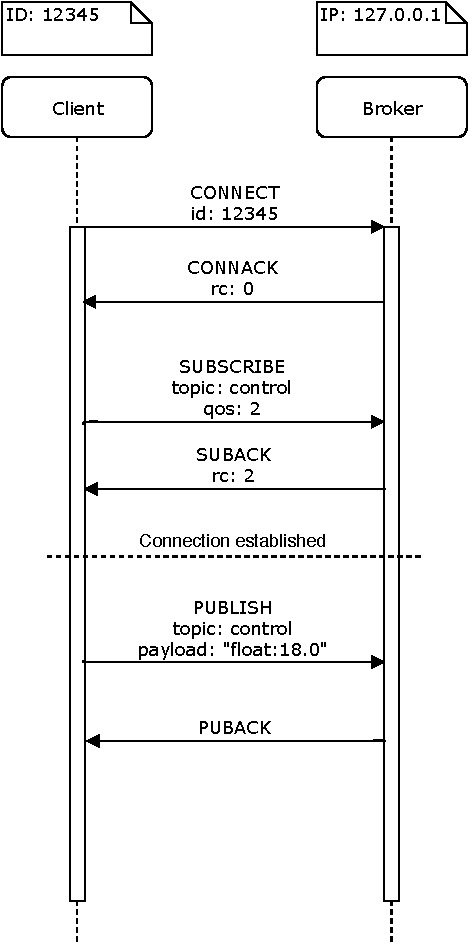
\includegraphics[width=0.5\textwidth]{obrazky-figures/MQTT-flow.pdf}
 \caption{Ukázka komunikace Klientu a Brokeru.}
 \label{mqtt-flow}
\end{figure}

\chapter{Návrh simulátoru}
\label{chap:arch-simul}

V~této kapitole se popisuje návrh vytvořeného simulátoru Petriho sítí, založeného na použítí knihovny SNAKES a simulující Petriho sítí v~reálném čase.

\section{Obecný návrh}

Simulace funguje na základě opakování dvou simulačních cyklu, jak je to popsané v~algoritmu \ref{real-time-alg}. První čeká na příchod nové události od plánovače, když ten druhý čeká na čas spouštění nejdřívější události ze seznamu plánovače.

Simulator se tedy sestavuje ze třech častí:

\begin{itemize}
  \item Plánovač události
  \item Simulace Petriho sítí
  \item Komunikace (MQTT)
\end{itemize}

Obrázek \ref{fig:sim-arch} vizualizuje strukturu častí simulátoru.

\begin{figure}[htb]
  \centering
  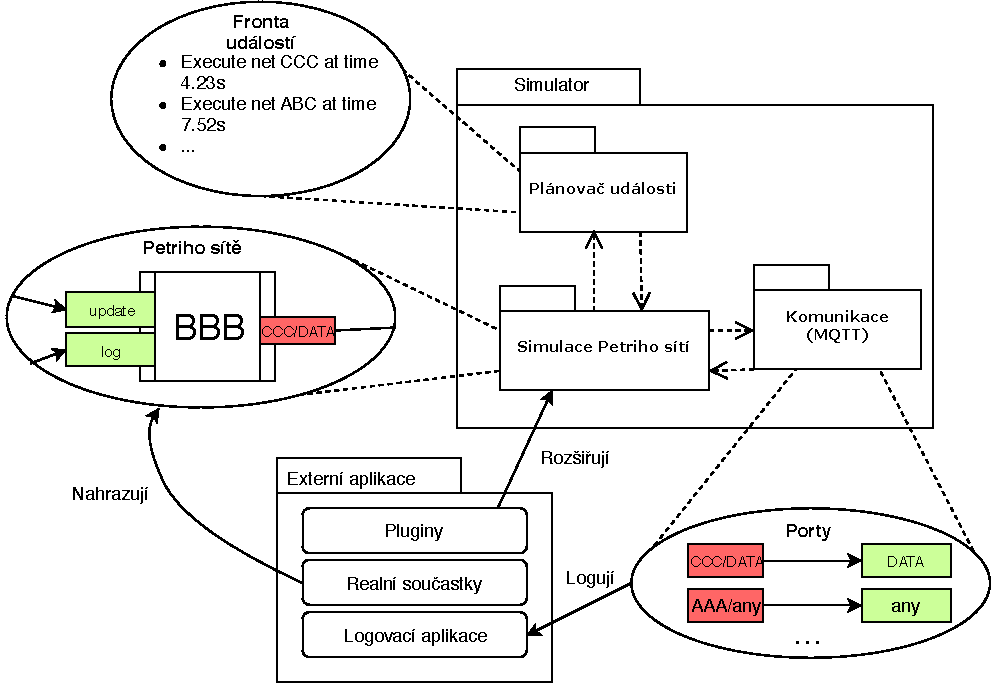
\includegraphics[width=0.85\textwidth]{obrazky-figures/sim-arch.pdf}
  \caption{Architektura simulátoru.}
  \label{fig:sim-arch}
\end{figure}

\section{Plánovač události}

Plánovač události je základem celého simulátoru. Na něm spočívá všechna činnost spojená s~plánováním spouštění sítí, blokováním a odblokováním simulační smyčky ve případě změn obsahu jeho plánovací fronty. To umožní provádění simulace v~reálném čase, a taky zabraní zbytečnému využití procesorového času ve chvíli když simulátor není obsazen vykonáváním nějaké úlohy.

Naplánované události se musejí ukládat do prioritní fronty v~deterministickém pořadí, a obsahovat časovou znáčku, podle které se určí, která událost se vykoná první.

\section{Simulace Petriho sítí}

Součásti simulátoru musí byt logická část, zaměřena na provádění Petriho sítí. Provádění se musí řídit plánovačem události, který spouští jejích provedení. Taky simulator musí mít možnost v~libovolný okamžik běhu naplánovat spouštěni Petrího sítí do plánovače události.

Taková simulace musí byt rozšířitelná a nahraditelná externími aplikacemi a rozšířeními pro účel nahrazení simulace realitou, a pozorovaní stavu běžících častí.

\section{Komunikační protokol}

Pro podporu simulací distribuovaných systému je potřeba použít protokol komunikaci, vhodný pro takové účely. Vzhledem k~zaměření tohoto simulátoru na vestavěné systémy, by implementace neměla být náročná na technické vybavení počítače. MQTT protokol je v~tom případě dobrou volbou.

Jeho cílem je obsloužení portů Petriho sítě, registrovaní a odhlášení instancí simulátoru, a zajištění stability dynamické podstaty simulatoru.

\chapter{Implementace simulátoru}
\label{chap:implementation}

V~této kapitole se popíše implementace simulátoru podle návrhu z~kapitoly \ref{chap:arch-simul}.

\section{Implementace simulace Petriho sítí.}
\label{sec:PNSim-impl}

Tato sekce popisuje implementací simulátoru Petriho sítí.

\subsection{Knihovna \texttt{SNAKES}}

\href{https://www.ibisc.univ-evry.fr/~fpommereau/SNAKES/}{\texttt{SNAKES}} -- knihovna v~jazyce Python, která nabízí všechno potřebné pro definici a spouštěni několika variant Petriho sítí. Cílem knihovny \texttt{SNAKES} je nabídnout badatelům možnost rychle namodelovat nový nápad. Zvláštní vlastnosti knihovny \texttt{SNAKES} je možnost vytvářet barevné Petriho sítě s~použitím výrazů v~jazyce Python pro anotaci přechodu či vstupních nebo výstupních šipek. \cite{snakes}

Zvláštní vlastností \texttt{SNAKES} je možnost implementace vlastních rozšíření pro jednotlivé částí Petriho sítí, nebo přidání nových vlastností pro modelování jiných podtypu Petriho sítí. Tato vlastnost byla zvlášť použita v~této prací pro přidání rozšíření \ref{sec:plug-impl}, podporující vytváření Petriho sítí určených pro modelovaní distribuovaných systému. Použítí těchto rozšíření je povinné pro správnou práci všech častí simulátoru.

Tato knihovna leží v~základu implementace simulátoru, a poskytuje implementací takových prvků, jako \texttt{PetriNet}, \texttt{Place}, \texttt{Transition} a metody pro přenos tokenů pří provedení přechodu.

\subsection{Simulační cyklus}


Plánovač událostí se používá pro plánovaní spouštění sítě do budoucna. Jsou tří případy pro vložení záznamu pro spouštění sítě do plánovače. Může to být uživatelská akce, příchod tokenu do nějakého ze vstupních portů sítě, nebo událost od rozšíření, takových jako \texttt{timed\_pl} -- \ref{subsec:timed_pl}.

Vložení událostí spouštění sítě do plánovače se nejčastěji provádí ve chvíli příchodu tokenů do nějakého ze vstupních portů. Pro tento účel komunikační část implementace propaguje tu událost do simulátoru, který ve své řádě ji zpracovává a vkládá záznam pro spouštění sítě do plánovače.

Provádění Petriho sítě je záležitost metody \texttt{execute\_net}. Táto metoda seřazuje zapnuté přechody do skupin podle priority, a následně je spouští. Taky se provádí seřazení uvnitř každé skupiny pro deterministické chovaní simulátoru. Provádění Petriho sítě je ukončené odesláním shromážděných tokenů z~výstupních portů podle popisu v~\ref{subsec:token-format}.

Čekání na čas spouštění sítě z~algoritmu \ref{real-time-alg} je naimplementovano metodou \texttt{sleep}.

Původní návrh simulátoru předpokládal že simulace bude běžet nějakou omezenou časovou dobu, ale to se ukázalo byt nepoužitelné pro případ využití v~teorii distribuovaných systémů. Takže současný stav simulátoru očekává ukončení simulaci příjetím signálu \texttt{SIGINT} nebo \texttt{SIGTERM} od uživatele.

\section{Implementace komunikace}
\label{sec:mqtt_impl}

Pro implementací MQTT klientu v~simulátoru byla použitá knihovna \href{https://pypi.org/project/paho-mqtt/}{\texttt{paho-mqtt}}. Tato knihovna obsahuje všechno potřebné pro nastavení komunikačních kanálů mezi porty vzdálených Petriho sítí. Na základě použití této knihovny konečný uživatel může nastavit zvolené místo v~Petriho sítí jako vstupní nebo výstupní port pomoci \ref{code:remote-in-out}. Jejích vzhled a nastavení je popsáné v~subsekci \ref{subsec:remote-ports-setup}.


\subsubsection{Směřování}
\label{subsec:mqtt-routing}

Na jeden vstupní port může být připojeno 0 až několik výstupních portů, nebo jinými slovy vstupní port přijímá všechny zprávy na svoje téma.

\begin{figure}[htb]
  \centering
  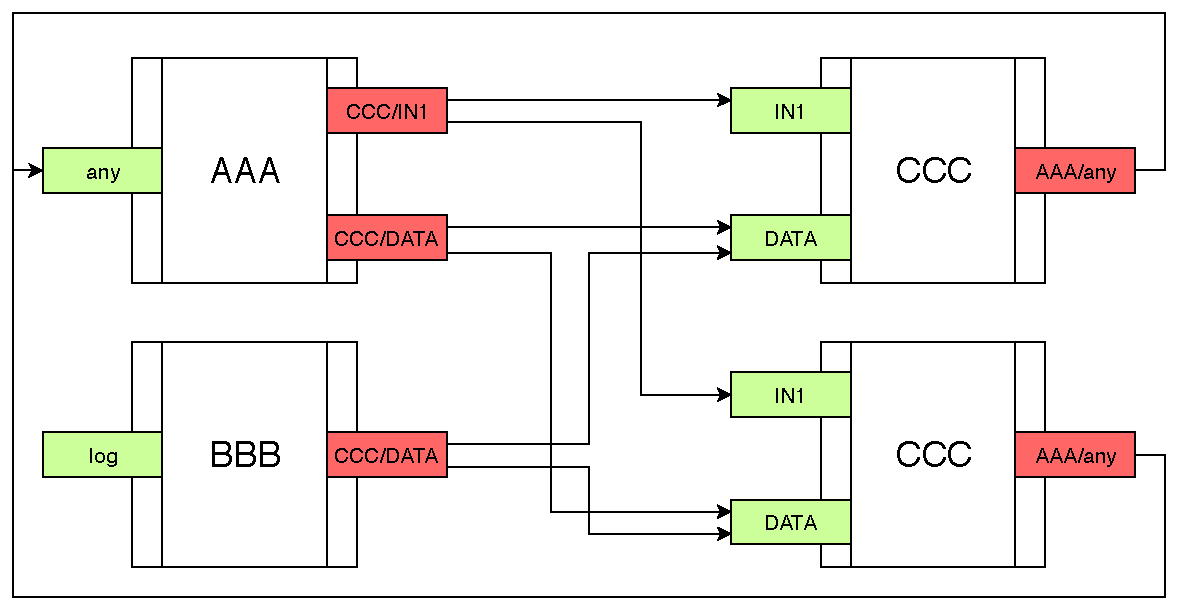
\includegraphics[width=0.7\textwidth]{obrazky-figures/Port-routing.pdf}
  \caption{Ukázka směřování zpráv.}
  \label{route-viz}
\end{figure}

Na výše dané obrázku \ref{route-viz} můžete vidět ukázku směrování zpráv mezi porty. \texttt{AAA}, \texttt{BBB} a \texttt{CCC} jsou identifikátory Petriho sítí v~rámci jediného brokeru. V~případě, že se dvojice síť--port  vyskytuje vícekrát, zprávy se přeposílají všem instancím. To si můžete všimnout na příkladu sítě \texttt{CCC}, která je na obrázku \ref{route-viz} dvakrát.

Na obrázku je 6 vstupních portů a 5 výstupních. Vstupní porty jsou označené zeleně, výstupní červeně. Jak je vidět na příkladě dvojic \texttt{CCC/IN1} a \texttt{CCC/DATA}, dvojice nemusí být unikátní. Počet připojených výstupních portu k~jednomu vstupnímu není nijak omezen. Je to dosažené použitím vlastností MQTT klientu popsané v~\ref{par:topic}. Stejně tak, počet vstupních portu přípojených k~jednomu výstupnímu, může být libovolný. Ukázkou je výstupní port jedné z~instanci sítí \texttt{CCC}, který je napojený hned na dva vstupní -- \texttt{AAA/any} a \texttt{BBB/update}. To umožňuje posílaní tokenů hned několika příjemcům.

Na příkladě vstupního portu \texttt{log} můžete vidět, že není povinné, aby port byl zapojený. V~případě simulátoru se chování vstupního portu s~takovým nastavením  neliší od už připojeného -- pokračuje v~naslouchání na svoje \uv{téma}. Pokud ale nějaký z~výstupních portů nebude mít žádnou registrovanou dvojicí, \uv{\texttt{NET/TOPIC}}, tak jenom zahazuje tokeny namísto odesílání. Víc o~použítí takového nastavení viz. \ref{subsec:external-app}.

Více se o~nastavení portů viz \ref{subsec:sim_pl} a \ref{subsec:remote-ports-setup}.

\subsection{Nastavení vstupních a výstupních portů}
\label{subsec:remote-ports-setup}

Na rozdíl od ostatních míst sítě, se vstupní a výstupní porty označují barvou a dodatečným popisem.

Je předem definované, že každá simulační instance odebírá zprávy z~tématu \texttt{control}. Je to ekvivalent broadkastové adresy pro nastavení. Pak každá instance simulátoru má svůj vlastní instanci MQTT klientu, id kterého se používá pro osobní zprávy určené instanci. Téma kterou odebírá instance je \uv{\texttt{private/<MQTT-CLIENT-ID>}}. Nastavení ostatních tématu je práce pro uživatele a je popsána v~dale.

\paragraph{Nastavení vstupního portu}

Běžná činnost pro vstupní port -- naslouchání na téma uvedené v~vizualizací portu. Seznam takových témat se nachází pod navěštím \texttt{Listening to}. Vstupní port se označuje zeleně. Výsledek je na obrázku \ref{port-in}.

\begin{python}
  # Vytvoreni site, mista a pridani ho do site
  n = PetriNet('CCC')
  p = Place('DATA')
  n.add_place(p)
  # Nastaveni portu 'data' jako vstupni port z~'CCC/DATA'.
  # Port DATA ze site CCC bude nastaven jako vystupni
  n.add_remote_input(p, 'CCC/DATA')
\end{python}


\begin{figure}[hbt]
 \centering
 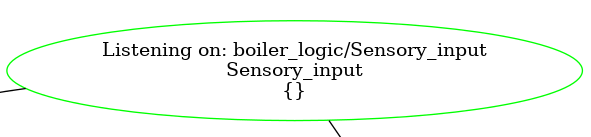
\includegraphics[width=0.35\textwidth]{obrazky-figures/port-in.png}
 \caption{Příklad vstupního portu}
 \label{port-in}
\end{figure}

\paragraph{Nastavení výstupního portu}

Činnost výstupního portu -- odesílaní všech tokenů z~napojeného místa po ukončení provedení sítě do témat ze seznamu uvedenému pod návěštím \texttt{Sending to}. Výstupní port se označuje červeným rámcem, a taky ve své reprezentací obsahuje seznám míst, kam se odešlou tokeny po ukončení provádění sítě. Výsledek nastavení je na obrázku \ref{port-out}.

\begin{python}
  # Vytvoreni site, mista a pridani ho do site
  n = PetriNet('CCC')
  p = Place('OUT')
  n.add_place(p)
  # Nastaveni portu 'OUT' jako vystupni port do 'AAA/any' a 'BBB/update'.
  # Porty 'any' a 'update' ze site 'AAA' a 'BBB' budou nastaveny jako vstupni porty.
  n.add_remote_output(p, 'AAA/any')
  n.add_remote_output(p, 'BBB/update')
\end{python}


\begin{figure}[hbt]
  \centering
  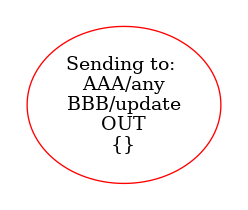
\includegraphics[width=0.35\textwidth]{obrazky-figures/port-out.png}
  \caption{Příklad výstupního portu}
  \label{port-out}
\end{figure}


Implementace zevnitř vypadá podobně reprezentací samotných portů. Síť, pří volání metody \texttt{add\_remote\_input} nastaví typ místa na vstupní, pak pošle zprávu na téma \texttt{control} obsahující dvojicí \texttt{[jméno sítě, jméno místa]} a uloží zprávu do čekací fronty. Pak, když se k~brokeru přípojí nějaká simulační instance s~požadovanou dvojicí síť--místo, zpráva se přepošle všem simulačním instancím. To se zase provede zasíláním zprávy na téma \texttt{control}. Hned po přijetí takové zprávy, port se nastaví a začne vykonávat svou činnost.

\subsection{Vlastní protokol komunikace}
\label{subsec:comm-proto}

Proto, aby simulátor měl podporu přidání vzdálených portů zmíněných v~\ref{sec:mqtt_impl} a registrací externích aplikací v \ref{subsec:external-app}, vznikla potřeba vymyslet vlastní protokol výměny informací mezi instancemi. Tento protokol musí mít seznam zpráv pro takové simulační případy, kdy port musí předat nebo přijmout tokeny nebo když se objeví instance Petriho síti v~nějakém z~již už existujících či nově vytvořených simulačních uzlů. Návod pro vytvoření takového je v~\ref{subsec:sim_pl}.

Následující tabulka \ref{tab:mqtt-msg-types} obsahuje přehled typů zpráv, a jejich formátu pro naplnění:

\begin{table}[H]
  \vskip6pt
  \caption{Tabulka typů zpráv}
  \vskip6pt
  \centering
  \begin{tabular}{lllr}
    \toprule
    Typ & Zkrátka & Formát \\
    \midrule
    Update & U~& \texttt{U\_ACTION, MQTT\_ID, NEW\_NET\_NAME} \\
    Request & R & \texttt{R\_ACTION, TARG\_NET/TARG\_PLACE, SRC\_NET/SRC\_PLACE} \\
    Success & S~& \texttt{REQUEST\_COPY} \\
    Failure & F & \texttt{REQUEST\_COPY, CUSTOM\_INFO} \\
    \bottomrule
  \end{tabular}
  \label{tab:mqtt-msg-types}
\end{table}

\subsubsection{Update}

Zprávy tohoto typu oznamují instancím simulátoru, jestli se v~jejich okolí neobjevila nová Petriho síť nebo naslouchající aplikace. Pomocí tohoto typu zpráv se provádí oznámení jiným simulačním instancím, že byla ukončena existence už registrovaných Petriho sítí. Takový případ může nastat, když byla nějaká simulace vypnuta zásahem uživatele.

\paragraph{Vytvoření simulace}

V~případě dodání zprávy typu \uv{Update} obsahující \texttt{U\_ACTION} nastavenou na hodnotu \uv{\texttt{update\_nets}}, taková zpráva bude sloužit k~oznámení vzniku nové instance simulace. Proto od té chvíle každá síť bude muset aktualizovat seznám vzdálených Petriho sítí a aktivních portů. V~případě, že nějaký port čeká na nastavení, tak dalším krokem se odešle požadavek na jeho nastavení. Poslední akcí je aktualizace tabulky známých vzdálených sítí u~nové instance simulací, předané zprávou na téma \texttt{private/<mqtt\_id>}, což je aproximací osobního kanálu spojení.

\begin{tabbing}
  \label{update-example}
  Příklad: \= \\
  \>\texttt{"U, update\_nets, 1, A\&B"}
\end{tabbing}

Hodnota \uv{\texttt{MQTT\_ID}} v~\ref{update-example} reprezentuje unikátní identifikační číslo instanci MQTT klientu. Takové číslo je důležité pro zpětnou aktualizaci seznamů známých Petriho sítí na stráně odesílatele. \uv{\texttt{NEW\_NET\_NAME}} jsou názvy Petriho sítí, oddělené znakem \uv{\texttt{\&}}. Výsledný tok nastavení můžete vidět na obrázku \ref{sim-register-viz}.

\begin{figure}[hbt]
  \centering
  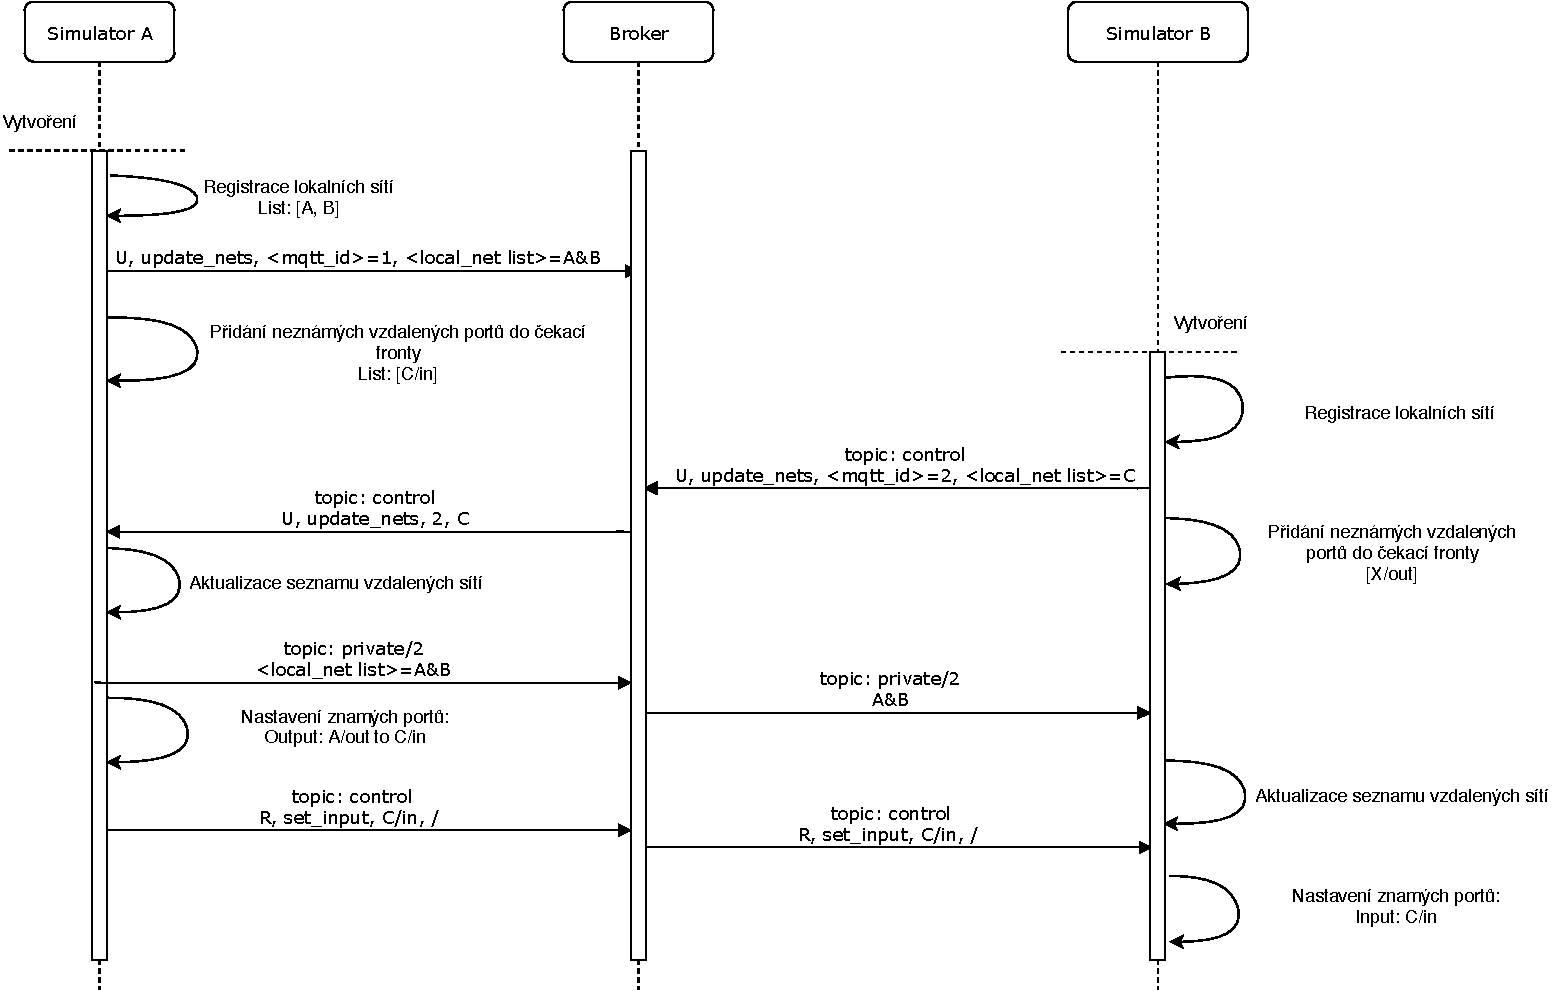
\includegraphics[width=1\textwidth]{obrazky-figures/sim-register.pdf}
  \caption{Vznik nové instancí simulace v~okolí brokeru.}
  \label{sim-register-viz}
\end{figure}

Stojí za zmínku, že \texttt{<mqtt\_id>} se nastaví pro simulaci ve chvíli, kdy bude vytvořena, a skládá se z~hašované hodnoty názvů lokálních Petriho sítí, které jsou součásti instance. Takže pokud nějaká simulace byla spuštěna vícekrát v~jeden okamžik, tak jejich chování bude zcela identické.

\paragraph{Ukončení simulace}

Když se provádí ukončení simulace, tak je důležité oznámit ostatním simulacím, že Petriho sítě, patřící do instance, budou taky vymazány. Takové chování zamezí zbytečnému odeslání tokenů na už neexistující porty, ale nezruší jejich nastavení. Ve chvíli, kdy takový výstupní port nebude mít kam odesílat tokeny, tak je začne zahazovat, aby se nehromadily ve výstupním místě. Více o~takovém nastavení viz. \ref{subsec:mqtt-routing}.

\begin{tabbing}
  \label{remove-example}
  Příklad: \= \\
  \>\texttt{"U, remove\_nets, 1, A\&B"}
\end{tabbing}

Hodnota \uv{\texttt{U\_ACTION}} je ve případě \ref{remove-example} nastavená na \uv{\texttt{remove\_nets}}, což po zpracování takové zprávy vymaže sítě \uv{\texttt{A}} a \uv{\texttt{B}}, ze seznamů vzdálených sítí na straně příjemce. Tok provedení této operací je zobrazen v~\ref{sim-unregister-viz}.

\begin{figure}[hbt]
  \centering
  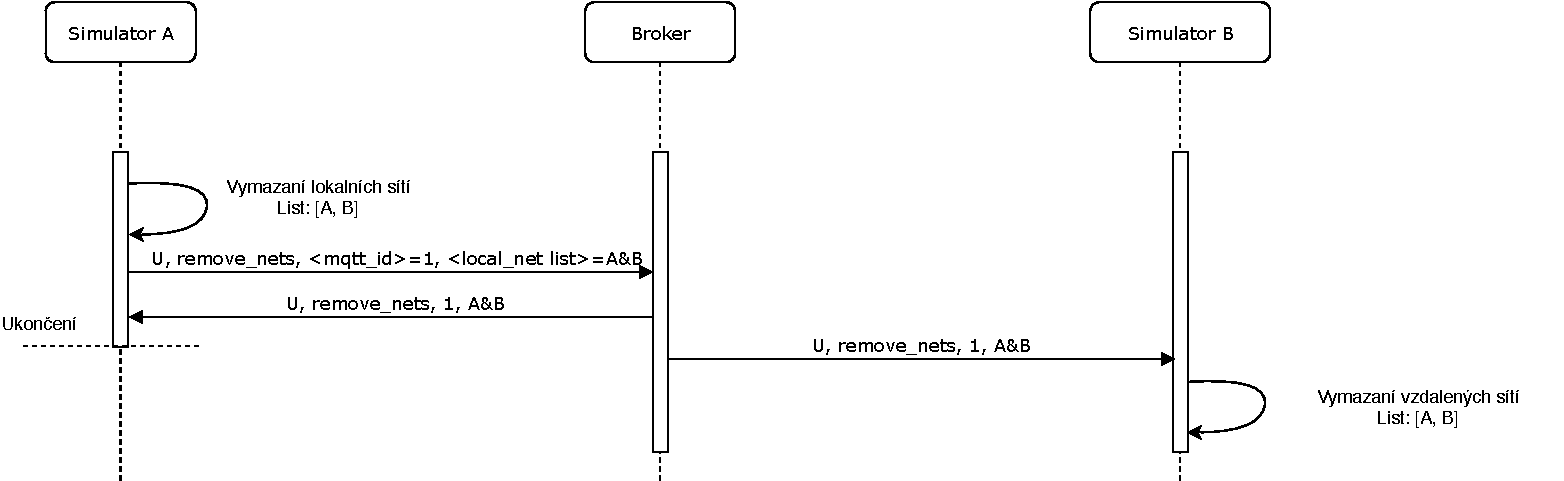
\includegraphics[width=1\textwidth]{obrazky-figures/sim-unregister.pdf}
  \caption{Ukončení existence simulační instance.}
  \label{sim-unregister-viz}
\end{figure}

\subsubsection{Request} \label{par:request} Tento typ zpráv nastavuje vstupní a výstupní porty. Parametr \uv{\texttt{R\_ACTION}} může nabývat hodnoty \texttt{set\_input} pro nastavení cílového místa \uv{\texttt{TARG\_PLACE}} jako vstupní port pro síť \uv{\texttt{TARG\_NET}}. Parametr \uv{\texttt{SRC\_NET}} a \uv{\texttt{SRC\_PLACE}} není v~tom případě potřeba, stačí uvést rozdělovač.

\begin{tabbing}
  Příklad: \= \\
  \>\texttt{"R, set\_input, net1/port1, /"}
\end{tabbing}

Pro nastavení výstupního portu stačí nastavit parametr \uv{\texttt{R\_ACTION}} na \texttt{set\_output} a dodat zdrojové místo a síť nastavením parametrů \uv{\texttt{SRC\_NET}} a \uv{\texttt{SRC\_PLACE}}.

\begin{tabbing}
  Příklad: \= \\
  \> \texttt{"R, set\_output, net1/port1, net2/port2"} \\
\end{tabbing}

\subsubsection{Success} Tato zpráva se odesílá ve případě úspěšného zpracování nějakého požadavku z~\ref{par:request}. Parametr \uv{\texttt{REQUEST\_COPY}} musí být přesnou kopií příchozího požadavku.

\begin{tabbing}
  Příklad: \= \\
  \> \texttt{"S, R, set\_output, net1/port1, net2/port2"} \\
\end{tabbing}

Přijetí, odesílající stranou potvrzovací zprávy Success, znamená že nastavení bylo úspěšné alespoň v~jednom případě, což má za následek nastavení místa s~jménem \texttt{port1} sítě \texttt{net1} jako výstupní port do \texttt{net2/port2}.

\subsubsection{Failure} Během zpracování nějakého požadavku z~\ref{par:request} může nastat chyba, o~které pomocí tohoto typu zprávy se dozví všechny instance simulace. Taková chyba ukončí všechny instance simulací a vypíše chybové hlášení. Parametr \uv{\texttt{REQUEST\_COPY}} musí být přesnou kopii příchozího požadavku. Parametr \uv{\texttt{CUSTOM\_INFO}} může obsahovat libovolnou zprávu.

\begin{tabbing}
  Příklad: \= \\
  \> \texttt{F, R, set\_output, net1/port1, net2/port2, }\\
  \> \texttt{Error: place "port1"\space was not found in net "net1"} \\
\end{tabbing}

Běžně se takové chyby vyskytují jenom ve fází vývoje aplikace, když uživatel zkouší přidávat nové Petriho sítě, takže nehrozí, že výsledná aplikace, nasazená do provozu, najednou spadne s~podobným chybovým hlášením.

\subsection{Využití protokolu pro registrací externích aplikaci.}
\label{subsec:external-app}

Vzhledem k~tomu, že simulace bez pozorování její stavu nemá smysl, celá předchozí sekce \ref{subsec:comm-proto} je navržena tak, aby libovolná externí aplikace byla schopna aplikovat popsané postupy pro navázaní spojení s~simulačními instancemi. Jediný požadavek v~tom případě je to, že aplikace se musí tvářit jako Petriho síť, která má vstupní nebo výstupní port. Tedy postup pro navázaní spojení je následující:
\begin{itemize}
  \item Připojit se k~MQTT brokeru, se kterým komunikuje pozorovaná skupina simulačních instanci.
  \item Poslat zprávu typu \uv{\texttt{Update}} na téma \uv{\texttt{control}}, obsahující seznám názvu sítí, které z~pohledu simulačních instancí bude obsluhovat navržená aplikace. Příklad takové zprávy je registrace žurnálová aplikace: \texttt{"U, update\_nets, 1234, logger"}, kde \uv{\texttt{logger}} je její název. Z~pohledu simulací se jedna o~Petriho síť.
  \item Nastavit porty simulací pro přijetí nebo odeslání tokenů pomoci zprávy typu \uv{\texttt{Request}} na téma \uv{\texttt{control}}: \texttt{"R, set\_output, kitchen-temperature-updater/Inside update, logger/kitchen"}.
\end{itemize}

Po uplatnění předchozích kroků, aplikace bude schopná přijímat tokeny z~místa \uv{\texttt{Inside update}} sítě \uv{\texttt{kitchen-temperature-updater}}. Tokeny mají gramatiku popsanou v~\ref{subsec:token-format}. Takové tokeny se budou posílat na téma \uv{\texttt{logger/kitchen}} po každém provedení sítě. Více o~takové aplikaci viz. \ref{sec:external-app-example}.

\subsection{Formát přenášených tokenů}
\label{subsec:token-format}

Simulator přeposílá tokeny ve tvaru textových řetězců \uv{\texttt{type:value}} oddělených znakem \&. Ve případě seznamů nebo množin, každá z~podmnožin takového prvku bude zakódovaná podobně jednotlivému tokenu, ale struktura seznamu bude zachovaná. Každá externí aplikace by měla dodržovat tuto syntaxi, aby simulator byl schopny zpracovat příchozí tokeny.

Syntaxe v~BNF je následující:
\begin{enumerate}
  \item $<TOKENLIST> :== <SUBLIST> \:\vert\: \epsilon$;
  \item $<SUBLIST> :==  <TOKEN> \:\&\: <SUBLIST> \:\vert\: <TOKEN>$
  \item $<TOKEN> :== <TYPE>:<VALUE> $;
  \item $<TYPE> :== int\:\vert\:float\:\vert\:string\:\vert\:bool\:\vert\:list\:\vert\:set $;
  \item $<VALUE> :== string$;
\end{enumerate}

\section{Implementace rozšíření}
\label{sec:plug-impl}

Tento oddíl popisuje implementaci různých rozšíření pro knihovnu \texttt{SNAKES}, které znesnadňují návrh Petriho sítí a jejího modelování. Každý z~níže popsaných pluginů se dá použít po jejich importu podle tohoto \href{https://www.ibisc.univ-evry.fr/~fpommereau/SNAKES/first-steps-with-snakes.html}{návodu}.

\subsection{Plugin \texttt{timed\_pl}}
\label{subsec:timed_pl}
Toto rozšířeni používá plánovač události pro spolehlivé plánovaní spouštěni přechodu do budoucna. Toto rozšíření používá jednoduchou logiku pro provedení přechodu -- ve chvíli, kdy přechod bude spustitelný, tak se zapne časovač a zkonzumuje odpovídající tokeny ze vstupních míst. Čekání se neresetuje přidáním dalších tokenů do vstupních míst. V~případě této implementace přechod vezme nově příchozí tokeny, které se objeví ve vstupních místech a tím zapnou přechod. Po ukončení čekání, bude nová skupina tokenů vložena do výstupních míst s~následujícími úpravami, které mohou nastat podle definice HLPN \ref{subsec:hlpn}.


\begin{python}
  # Vytvoreni prechodu s~casovym zpozdenim
  pr1=Transition("Timed-transition", timeout=30) (*\label{code:timed-example}*)
\end{python}

Pro vytváření takového přechodu stačí zadat parametr \texttt{timeout} do klauzule pro vytvoření přechodu -- \texttt{Transition}, jak je ukázáno na řádku \ref{code:timed-example}. Hodnota \texttt{timeout} se uvádí v~sekundách. Výsledný tvar následujícího přechodu je na obrázku \ref{timed-transition}. Ukázku použítí ve funkčním příkladu můžete vidět \hyperref[code:timed-temp-example]{dále}.

\begin{figure}[hbt]
  \centering
  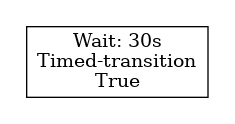
\includegraphics[width=0.3\textwidth]{obrazky-figures/timed-transition.png}
  \caption{Příklad časovaného přechodu}
  \label{timed-transition}
\end{figure}

\subsection{Plugin \texttt{prob\_pl}}
\label{subsec:prob_pl}
Toto rozšíření přidává možnost spojit několik přechodů do jedné skupiny, a tudíž rovnoměrně rozdělit pravděpodobnost spuštění každé z~nich. Pro spojené přechody platí, že musí mít stejnou sadu vstupních míst. Pak se při provedení jednoho z~nich rozhodne na základě hodnoty jeho pravděpodobnost, jestli se tento přechod musí provést, nebo se provede některý z~jeho sousedů. Součet pravděpodobnosti pro takovou skupinu přechodů musí být vždycky roven 1.

Takový přechod se definuje ve dvou krocích. Nejdříve se vytvoří prvek \texttt{Transition} s~parametrem \texttt{prob}, jak je ukázáno na řádku \ref{code:prob-example}. Příklad použití v~\hyperref[code:prob-ev-draw]{obecném} případě viz. řádek \ref{code:prob-temp-example}.
\begin{python}
  # Krok 1: Vytvoreni prechodu z~parametrem prob
  pr1=Transition("Prob-trans-1", prob=0.6) (*\label{code:prob-example}*)
  pr2=Transition("Prob-trans-2", prob=0.4)
\end{python}

Dále stačí spojit pravděpodobnosti přechodu do jedné skupin pomocí klauzule \\ \texttt{add\_neighbour\_transition}. Viz. řádek \ref{code:prob-neghb-example} nebo řádek \ref{code:prob-temp-neghb-example-1} z~kompletního \hyperref[code:prob-ev-draw]{příkladu}.
\begin{python}
  # Krok 2: Vytvoreni prechodu s~parametrem prob
  pr1.add_neighbour_transition(pr2) (*\label{code:prob-neghb-example}*)
\end{python}

Tato sekvence vytváří následující zobrazení -- \ref{prob-transition}.

\begin{figure}[hbt]
  \centering
  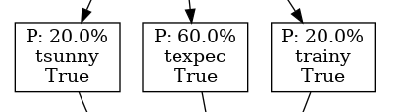
\includegraphics[width=0.6\textwidth]{obrazky-figures/prob-transition.png}
  \caption{Příklad pravděpodobnostního přechodu}
  \label{prob-transition}
\end{figure}

\subsection{Plugin \texttt{prior\_pl}}
\label{subsec:prior_pl}
Tento plugin je určený pro přidání prioritních pochodů do Petriho sítě. Podle nastavené priority se během simulace bude rozhodovat, který přechod se vyhodnotí a provede jako první. Priority mohou být v~rozsahu 0 -- 100, a řadí se sestupně. Pro nastavení priority element \texttt{Transition} má dodatečný a nepovinný parametr \texttt{prior} -- \ref{code:prior-transition-example}.
\begin{python}
  # Ukazka prioritniho prechodu
  tr=Transition('Enable boiler', prior=1) (*\label{code:prior-transition-example}*)
\end{python}

\begin{figure}[hbt]
  \centering
  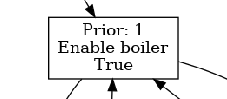
\includegraphics[width=0.3\textwidth]{obrazky-figures/prior-transition.png}
  \caption{Příklad prioritního přechodu s~prioritou $1$}
  \label{prior-transition}
\end{figure}

\subsection{Plugin \texttt{sim\_pl}}
\label{subsec:sim_pl}

Na implementací tohoto pluginu je založená práce ostatních pluginů ze skupiny \ref{sec:plug-impl}. Je ve své podstatě spojovacím prvkem mezi simulátorem, $MQTT$ klientem a Petriho sítí. Obsahuje přetěžovaní metod z~knihovny \texttt{SNAKES} pro vykreslování prvků, které jsou rozšířené pluginy. Taky přidává zásadní metody pro nastavení Petriho sítě, umožňující použití simulátoru a provádění spouštění sítě \ref{code:add_simulator}.
\begin{python}
  sim=PNSim() (*\label{code:sim-add}*)
  n=PetriNet("Sample net")
  n.add_simulator(sim) (*\label{code:add_simulator}*)
\end{python}

Stejně tak podporuje nastavení vzdálených portů pro předání tokenů jiným instancím simulátoru připojeným na stejnou adresu \texttt{MQTT} brokeru \ref{code:remote_in}, \ref{code:remote_out}.

\begin{python}
  n.add_remote_input(it, "temp_gen/Measurement") (*\label{code:remote_in}*) (*\label{code:remote-in-out}*)
  n.add_remote_output(hen, "boiler-logic/Sensory_input") (*\label{code:remote_out}*)
\end{python}

\subsubsection{Vykreslování stávu simulace}

Každá instance simulátoru dokáže vykreslit svůj původní a aktuální stav Petriho sítí do následující struktury složek -- \ref{fig:draw-stucture}.

Původní stav: \uv{\texttt{net-drawings/<název simulace>/starting/<net-name>.png}}

Současný stav: \uv{\texttt{net-drawings/<název simulace>/current/<net-name>.png}}.

\begin{figure}
  \centering
  \framebox[\textwidth]{%
  \begin{minipage}{0.9\textwidth}
    \dirtree{%
    .1 simulation-root.
    .2 net-drawings.
    .3 all-in-one.
    .4 starting.
    .5 net1.png.
    .4 current.
    .5 net1.png.
    .3 server.
    .4 starting.
    .4 current.
    }
  \end{minipage}
  }
  \caption{Struktura uložení zobrazení Petriho sítí.}
  \label{fig:draw-stucture}
\end{figure}

\subsection{Návod pro import rozšíření}
Vzhledem k~odlišnému postupu pří přidání rozšíření do SNAKES, pro import simulačního nástroje a dalších rozšíření ze skupiny, uživatel musí dodržovat správné pořadí při importu knihoven. Konvence probíhá následujícím způsobem.

\begin{python}
  from snakes.nets import *   # Site, mista, prechody... (*\label{code:snakes-all}*) (*\label{code:plugin-setup}*)
  from simul import PNSim     # Simulacni knihovna (*\label{code:pnsim}*)
  snakes.plugins.load( (*\label{code:sim-plugins}*)
  ["gv", "timed_pl", "sim_pl", "prob_pl", "prior_pl"],
  "snakes.nets",
  "plugins") # Seznam rozsireni pro import
  from plugins import * # Redefinovane metody z~rozsireni (*\label{code:pl-import}*)
\end{python}

\begin{enumerate}
  \item Přidání knihovny snakes a jejich prvků \ref{code:snakes-all}.
  \item Import simulační knihovny, která poskytne základ pro rozšíření \ref{code:pnsim}.
  \item Přidání rozšíření podle požadovaných vlastností sítě \ref{code:sim-plugins}. Ze skupiny doporučených pluginů stojí za zmínku plugin \href{https://www.ibisc.univ-evry.fr/~fpommereau/SNAKES/API/plugins/gv.html}{\uv{gv}}. Jeho implementace používá nástroj \href{https://www.graphviz.org/}{\texttt{GraphViz}} pro vytvoření vizuální reprezentace Petriho sítě. Více o~jeho použití v~rámci simulátoru viz. \ref{sec:mereni-teploty}. Zbytek je popsán v sekcích \ref{subsec:timed_pl}--\ref{subsec:sim_pl}.
  \item Pro redefinici a přidání nových metod z~rozšíření slouží řádek \ref{code:pl-import}. Od dané chvíle použití knihovny SNAKES je stejné jako v~\href{https://www.ibisc.univ-evry.fr/~fpommereau/SNAKES/first-steps-with-snakes.html}{návodu} a taky \ref{chap:postup}.
\end{enumerate}


\section{Plánovač události}
\label{sec:event-planner}

Plánovač události je naimplementován jako prioritní fronta za využiti vestavěné knihovny \href{https://docs.python.org/3/library/heapq.html}{\texttt{heapq}} v~jazyce Python. Api naznačuje, že pro přidání a výběr prvků se používají metody \texttt{heappush} a \texttt{heappop}. Priorita v~takové frontě se určuje číselnou hodnotou, která se vkládá do fronty. Tato hodnota může být prvním prvkem v~seznamu elementů. Druhým parametrem pro určení priority je pořadí, ve kterém byl prvek vložen. Tato sada pravidel umožňuje vkládat záznamy, obsahující čas spuštění jako první prvek, a podle toho se zařadí na příslušné místo ve řadě. Metoda \texttt{heappop} vybere prvek ze seznamu s~nejvyšší prioritou, což bude element s~nejnižší hodnotou času.

Pro účel plánování události se používají dvě funkce -- \texttt{schedule\_at} \ref{code:schedule-at} a \texttt{schedule} \ref{code:schedule}. Jedna slouží pro vkládání událostí na čas od začátku simulace, když ta druhá pracuje se současným časem simulace. Funkce jsou určeny pro počáteční spouštění sítí po přidání do simulátoru. Pro případ že by uživatel potřeboval provést operaci hned po vložení, bez porušení pořadí předchozích operací, je definovaná konstanta \pyth{PNSim.NOW}.

Záznamy musí odpovídat určitým zásadám, aby simulátor byl schopný takový záznam zpracovat. Každý záznam obsahuje ve své struktuře referenci na zvolenou funkci jako první prvek. Následující prvky seznamu jsou argumenty, které budou předány této funkci ve chvíli její vyhodnocení.

Ukázku takového záznamu můžete vidět na řádku \ref{code:event-struct}.

\begin{python}
  ev = [simul.execute_net, net.name] # Udalost a jeji argumenty (*\label{code:event-struct}*)
  # Planovani udalosti na soucasny okamzik.
  sim.schedule(event=ev, tm=PNSim.NOW, prior=0) (*\label{code:schedule}*)
  # Planovani udalosti na cas 15s od zacatku simulace.
  sim.schedule_at(event=ev, tm=15, prior=0) (*\label{code:schedule-at}*)
\end{python}

Pro účely vývoje simulátor vypisuje logy z~plánovače události do souboru \texttt{./planner.log'} ve složce, kde byl spuštěn.

\chapter{Aplikace -- návrh}
\label{chap:app-arch}

V~této kapitole je popsán návrh a implementace zvolené aplikace simulátoru -- chovaní řízení topení.

\section{Řízeni topení}
\label{sec:tepelne-rizeni}

Pro demonstraci práce simulátoru bylo rozhodnuto namodelovat distribuovaný systém modelující chování topení, který pravděpodobně používáte u~sebe doma. Takový systém se sestavuje z~několika částí. Základním prvkem je plynový spotřebič nebo bojler. Ten ohřívá vodu a uvádí ji do pohybu po potrubích. Pak každý z~pokojů ma na starosti tepelné čidlo a řízení, které udržuje v~pokoji nastavenou teplotu podle kalendáře teplot pro daný čas. Kazdou hodinu se z~tabulky teplot vezme aktuální teplota pro současnou hodinu a tento pokoj, pak řízení rozhodne jestli má zapnout topení nebo ne. Pokud žádný z~pokojů v~současné době nemá zapnuté topení, tak se karma musí vypnout za účelem šetření plynu. Toto řízení provádí vestavěný systém v~bojleru, protože je zcela mechanický. Každý z~těch prvků bude dále namodelován Petriho sítěmi. Pro pochopení struktury viz. \ref{boiler-net}.

\section{Struktura aplikace}

Návrh \ref{boiler-net} se sestavuje z~5 částí:
\begin{itemize}
 \item Řízení
 \item Sklep
 \item Obývací pokoj
 \item Kuchyně
 \item Vnější prostředí
\end{itemize}
Každá z~částí návrhu je zvláštní instance simulátoru. Taková instance může být spuštěna nebo pozastavena v~různou dobu a zcela nezávisle na jiných instancích simulátoru nebo jiných podmínkách.

Takové rozdělení se vysvětluje snahou napodobovat skutečné rozložení pokojů. Ve sklepě se nachází bojler, což je reprezentováno Petriho sítí zvané \uv{\texttt{Boiler}} a stav teploty toho pokoje se řídí svým vlastním mikropočítačem a jeho reprezentací je síť \uv{\texttt{Sklep: simulace prostředí}}. Skutečnou síť pro bojler můžete vidět na obrázku \ref{boiler-logic-viz}, a její popis je v~\ref{sec:boiler-net-details}.

Pak každý z~pokojů disponuje svou vlastní instancí simulátoru, která simuluje teplotní změny uvnitř pokoje.

Poslední, ale přesto nejdůležitější částí návrhu \ref{boiler-net}, je řízení pokojů. V~reálných podmínkách takové řízení se provádí na zvláštním serveru, což reprezentuje instance simulace, zvaná \uv{\texttt{Řízení}}. Její součásti jsou Petriho sítě, simulující chování čidel a ventilu radiátoru v~pokoji, jako \uv{\texttt{Kuchyně:
řízení ventilu}}, a taky tabulky očekávaných teplot pro daný čas \uv{\texttt{Tabulka teplot}}.

\begin{figure}[htb]
 \centering
 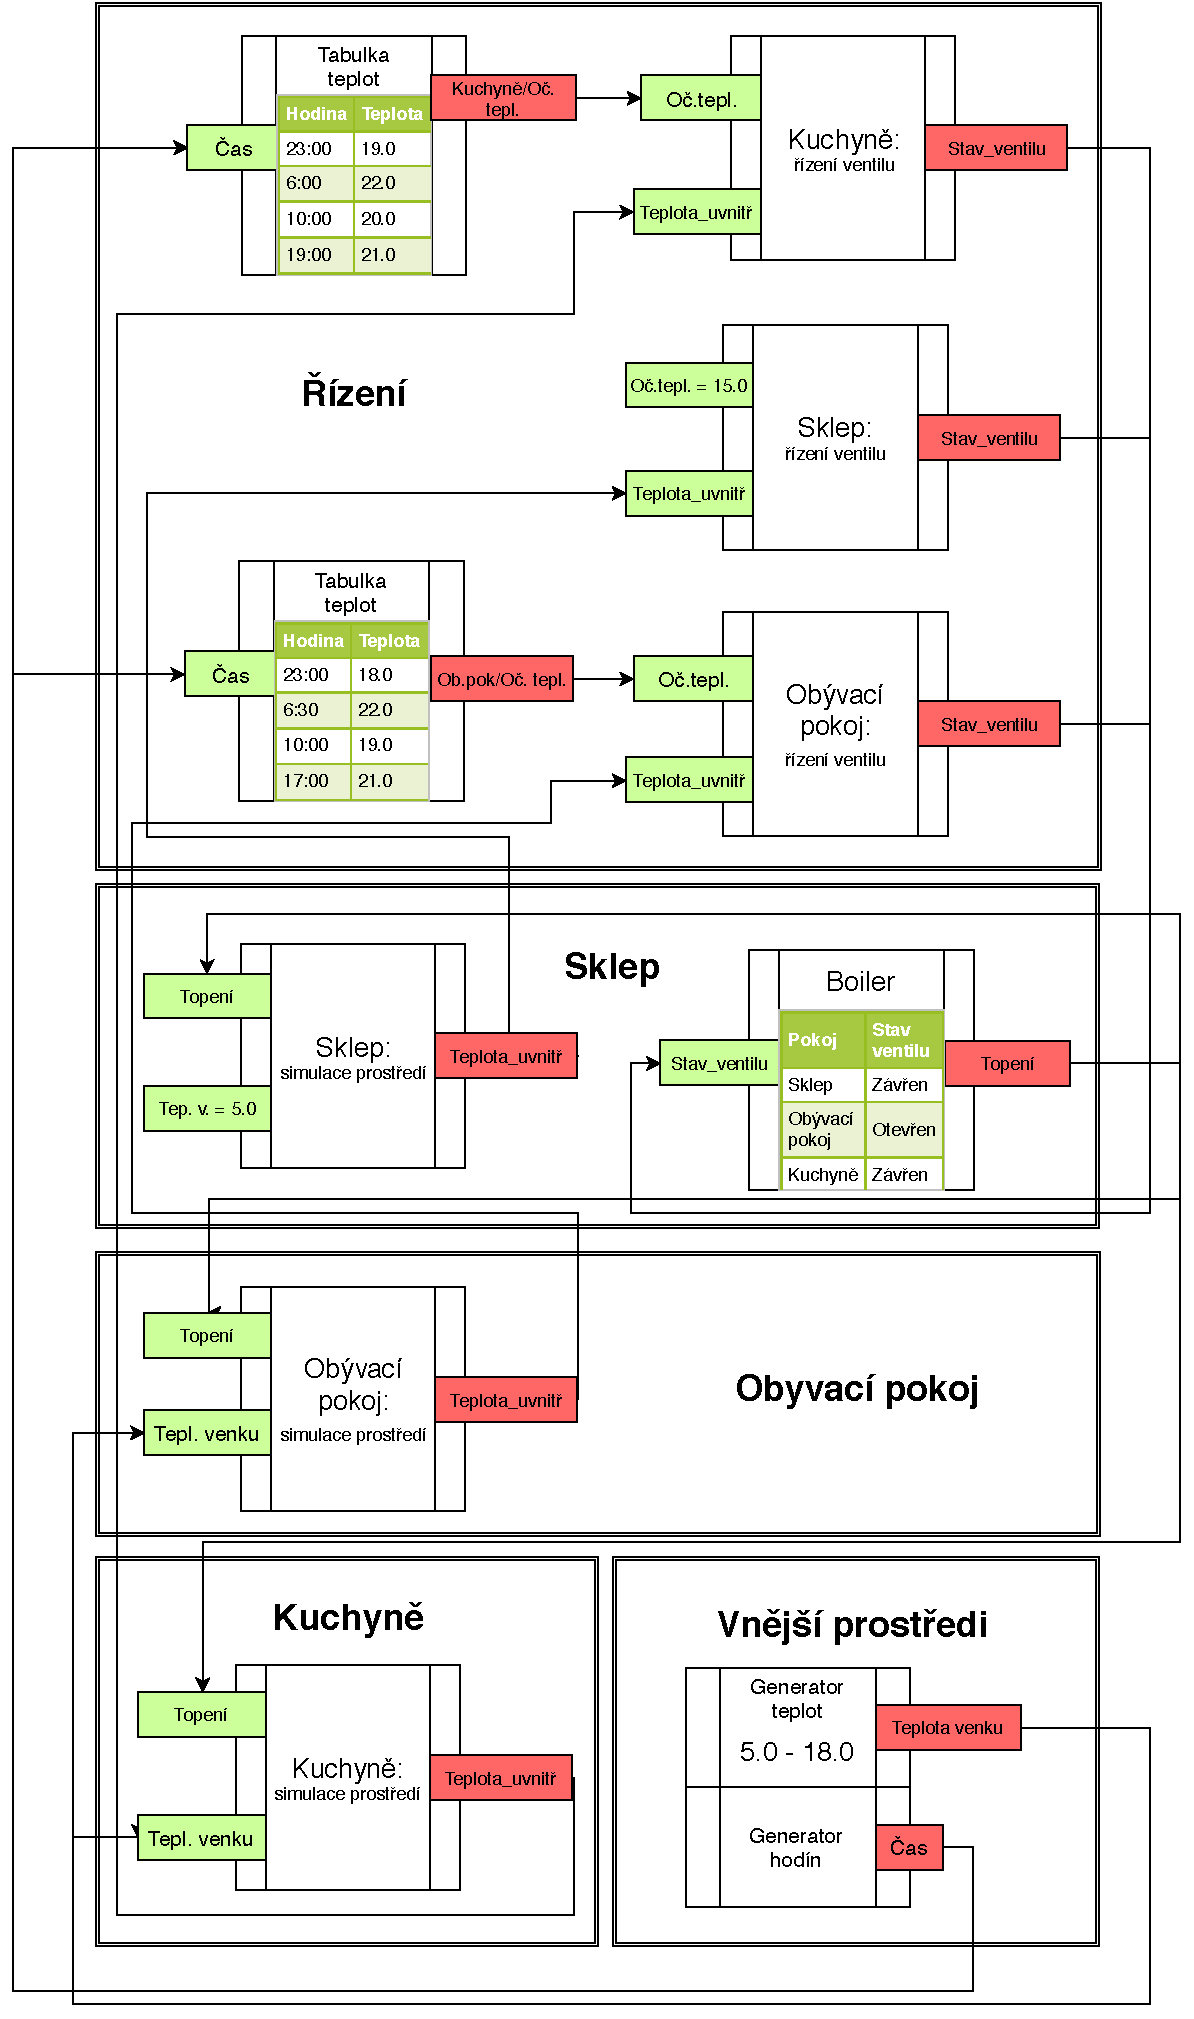
\includegraphics[width=0.85\textwidth]{obrazky-figures/boiler-net.pdf}
 \caption{Architektura aplikace}
 \label{boiler-net}
\end{figure}

Aby tento návrh, co nejpřesněji odpovídal realitě, bylo rozhodnuto, namodelovat chování teploty v~pokoji. Pro tento účel, například slouží síť ze simulační instance \uv{\texttt{Sklep}} pod názvem \uv{\texttt{Sklep: simulace prostředí}}.

Pro splnění tohoto úkolu nejdříve musíme vědět, jak výkonné je topení v~pokoji. Běžné hodnoty pro tři druhy pokojů můžete vidět v~následující tabulce \ref{tab:tepelne-ztraty}. Dále nás zajímají tepelné ztráty a taky množství energie potřebné pro ohřáti pokoje. Pro výpočet tohoto parametru použijeme následující vzoreček. Základním parametrem, rozhodujícím o~tepelné kapacitě pokoje, je plocha vnitřního povrchu pokoje $V$, respektive celková plocha povrchu stropu, podlahy a stěn. Pro ně je důležité vědět koeficient ztrát tepla $K$. Zvlášť se počítají okna a dveře, vzhledem k~jejich větší vodivosti tepla. Pak zbývá jenom zjistit rozdíl současné teploty uvnitř pokoje a očekávané teploty pro tuto hodinu -- $\Delta{T}$. To všechno dosadíme do vzorečku a zjistíme celkové množství energie, potřebné pro jeho ohřáti. \cite{tep_calc}
\begin{center}
 $Q[kW/h] = \frac{V*\Delta{T}*K}{860}$
\end{center}

Pak koeficienty vypadají následovně:

\begin{table}[H]
  \vskip6pt
  \caption{Tabulka parametrů pokojů}
   \vskip6pt
  \centering
  \begin{tabular}{lllr}
    \toprule
    Typ pokoje & Koeficient tepelných ztrát & Objem $[m^3]$ & Očekávaný výkon topení $[W]$ \\
   \midrule
   Kuchyně & 0.5 & $4*3*2.5$ & $1200$ \\
   Obývací pokoj & 0.6 & $6*4*2.5$ & $2300$ \\
   Sklep & 0.8 & $3*3*2.2$ & $300$ \\
    \bottomrule
  \end{tabular}
  \label{tab:Parametry}
\end{table}

Na výpočet tepelných ztrát pokoje jsem použil \href{https://wpcalc.com/kalkulyator-teplopoter/}{tento} nastroj.
Vychází to zhruba následovně:

\begin{table}[H]
  \vskip6pt
  \caption{Tabulka tepelných ztrát pokojů}
   \vskip6pt
  \centering
  \begin{tabular}{llr}
    \toprule
    Typ pokoje & Ztráty $[kW/h]$ \\
    \midrule
    Kuchyně & $0.7$ \\
   Obývací pokoj & $1$ \\
   Sklep & $0.4$ \\
    \bottomrule
  \end{tabular}
  \label{tab:tepelne-ztraty}
\end{table}

Celé chování systému odpovídá zákonu zachování energie, a tak můžeme odvodit rovnici pro výpočet jejího potřebného množství.

\chapter{Aplikace -- implementační detaily}
\label{chap:app-implementation}

V~této kapitole jsou detailně popsaný obrázky Petriho sítí, vygenerované během simulace, které umožňují simulaci senzorů teplotního řízení pokojů \ref{sec:server-details}, ohřívaní pokoje a převod energii na teplotu pokoje -- \ref{sec:room-sim-details}, a jiné.

\section{Simulace vnějšího prostředí}
Tato část aplikace je vyhrazena do zvláštních simulačních instanci, vzhledem k~tomu že není závislá na žádných jiných částech aplikace. Obsahuje jenom jednu síť ve svém zapouzdření -- Simulace počasí a času \ref{weather-viz}. Tato síť vytváří dvě podstatné věci pro tuto aplikaci, čas a teplotu pro tento čas. Podrobnější návrh a implementace je v~\ref{sec:mereni-teploty}.

\begin{figure}[htb]
 \centering
 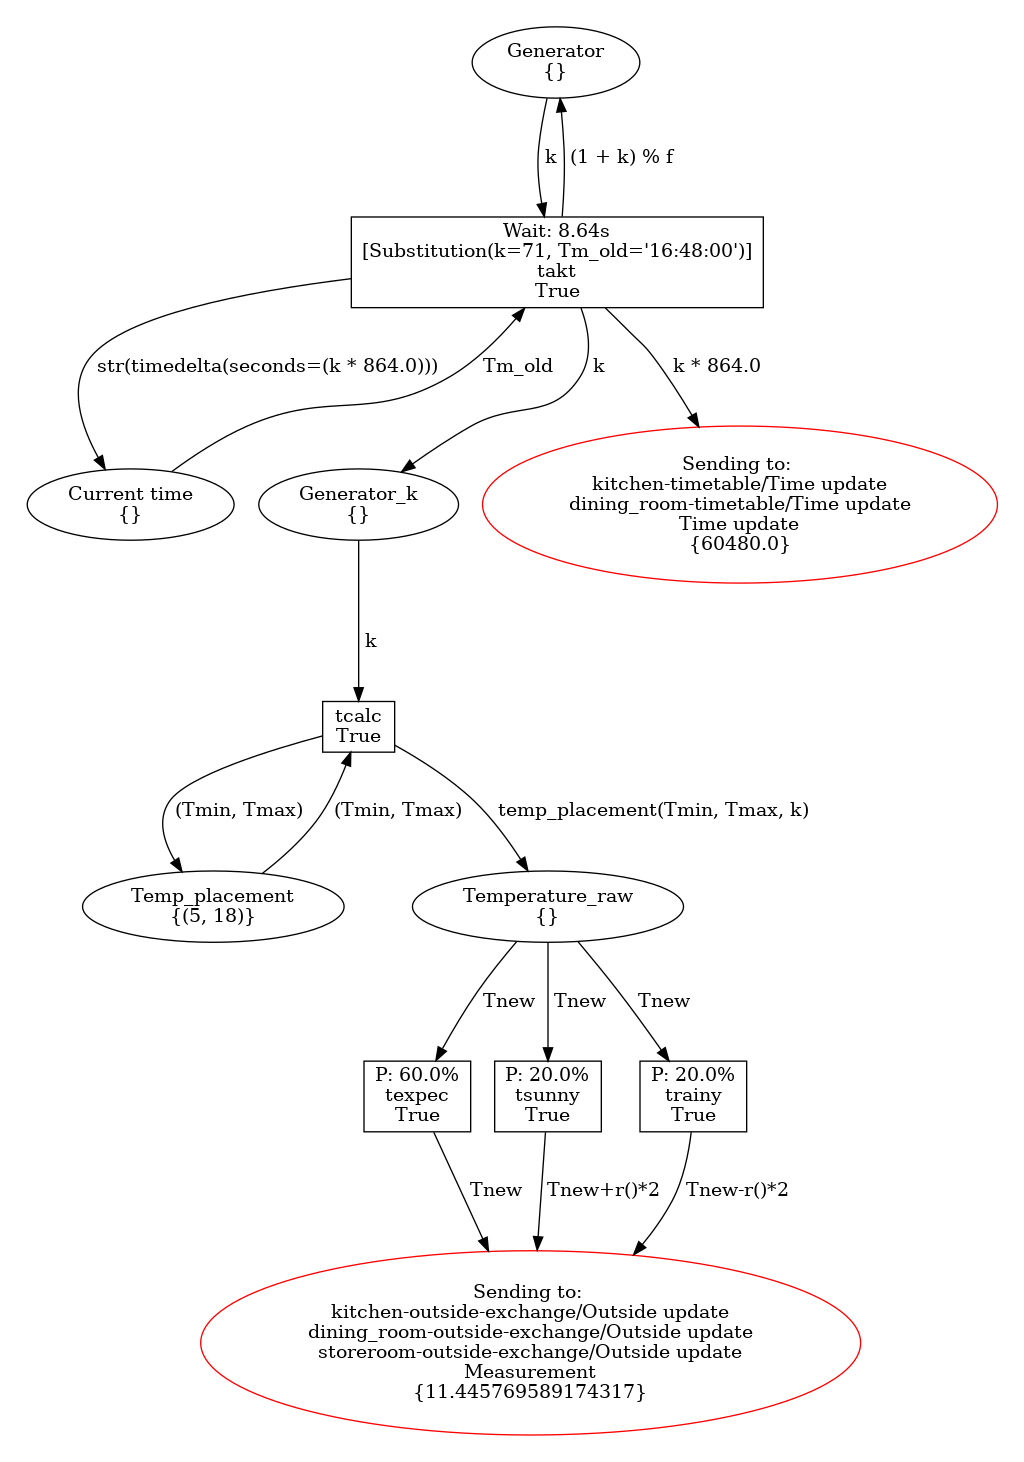
\includegraphics[width=\textwidth]{obrazky-figures/weather-sim.png}
 \caption{Simulace počasí a času.}
 \label{weather-viz}
\end{figure}

\section{Simulace pokojů}
\label{sec:room-sim-details}

V~rámci této simulace se popisuje chování řídícího systému senzoru a simuluje se chování teploty pro každý z~pokojů. Implementace kódu v~jazyce Python se dá najít \href{https://github.com/Danil-Grigorev/rt-sim-petry-net/tree/master/sample_nets}{tady}.

\subsection{Výměna energii se vnějším prostředím}
\label{subsec:energy-exchange}

Tato Petriho síť je jednou ze součásti simulace pokoje, a může být vyměněna za podrobnější a rozsáhlejší její variantu ve případě že přesnost simulace je bodem srázu. Její cílem je modelovat chování změny teploty v~pokoji během výměny teploty se vnějším prostředím. Pro tento účel slouží srovnání současné hodnoty teploty venku a vevnitř pokoje. První hodnota je uložena pro lokální využití v~místě s~názvem \uv{\texttt{Temperature outside}}. O~její aktualizaci se stará vstupní port \uv{\texttt{Outside update}}. Pro aktualizaci vnitřní teploty je vstupní port \uv{\texttt{Inside temp update}} a lokální hodnota se nachází v~\uv{\texttt{Temperature inside}}.

Výměna teploty se vnějším prostředím se provádí na základě pollingu každých $30$ vteřin, což se řídí časovanými přechody \uv{\texttt{Temperature gain}} a \uv{\texttt{Temperature loss}}. Výsledek provádění takového přechodu je vzorec, který spočítá kolík [W] energii bylo ztráceno nebo získáno během těch $30$ vteřin -- $q\_lps*exch\_time$. Hodnota $q\_lps$ je definovaná jako globální proměna v~prostředí Petriho sítě. Kód této sítě se nachází v~\href{https://github.com/Danil-Grigorev/rt-sim-petry-net/blob/master/sample_nets/temp_sensor.py}{souboru} \texttt{temp\_sensor.py}.

Výsledek můžete vidět na obrázku \ref{exchange-viz}.

\subsection{Převod změn energii na teplotu}

Tato síť spojuje hned několik častí simulace řízení teploty v~pokoji, a složí pro převod změn energii do stupnici Celsia. Každý z~pokojů má uloženou svou hodnotu v~místě \uv{\texttt{Q per C}}. Pokud do vstupního portu \uv{\texttt{Q change}} přichází změna energii ze sítí \ref{subsec:energy-exchange} nebo \ref{subsec:room-heating}, ta hodnota bude převedena do stupnici Celsia a přidá se do aktuální hodnoty teploty v~pokojí, uloženou v~místě \uv{\texttt{Temperature inside}}. Tato změna bude oznámena takovým častém simulací jako řízení -- \ref{subsec:room-control} přes výstupní port \uv{\texttt{Inside update}}.

Výsledná síť je v~\ref{room-temp-viz}.

\subsection{Simulace ohřívání pokoje}
\label{subsec:room-heating}

Tato část aplikace je taky vyhrazena do zvláštní instance Petriho sítě, a její cílem, simulace ohřívaní pokoje pří zapnutém bojleru a otevřeném ventilu v~pokoji. Informace o~stavu ventilu přichází do vstupního portu \uv{\texttt{Valve update}}. Stav bojleru přichází do \uv{\texttt{Heater update}}. Jejích lokální stavy se ukládají do míst \uv{\texttt{Heater state}} a \uv{\texttt{Valve state}}.

Samotné ohřívaní pokoje se provádí časovaným přechodem \uv{\texttt{Heating}}, který vkládá množství energii, vyprodukované radiátorem za dobu \uv{\texttt{heat\_time}} podle vzorečku $q\_gps * heat\_time$. Hodnota $q\_gps$ je definovaná pro každý z~pokojů zvlášť jako globální deklarace v~prostředí Petriho sítě. Výsledek  můžete vidět v~\ref{heater-viz}.

\begin{figure}[htb]
 \centering
 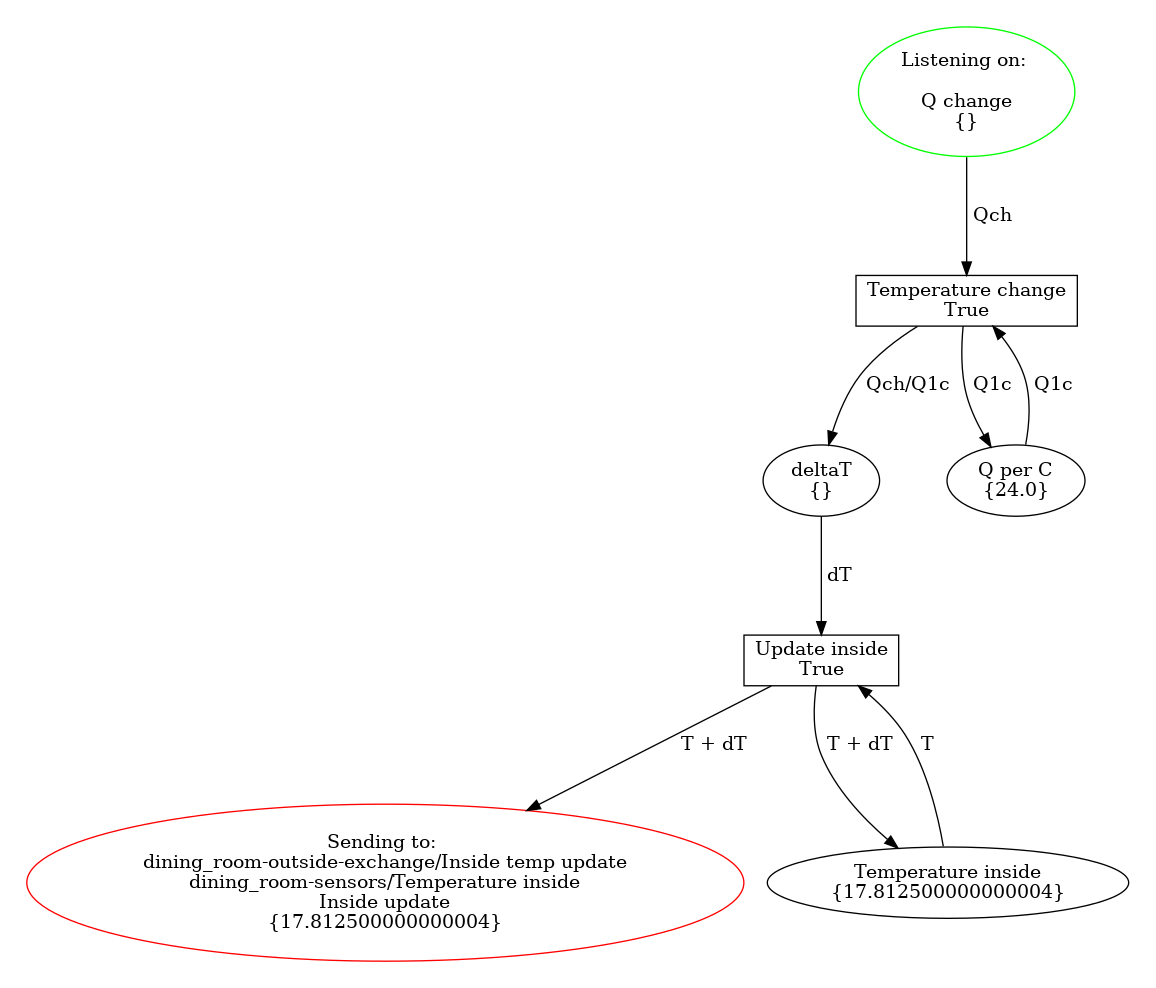
\includegraphics[width=\textwidth]{obrazky-figures/room-temp-upd.png}
 \caption{Převod energii na stupnici celsia.}
 \label{room-temp-viz}
\end{figure}

\begin{figure}[htb]
 \centering
 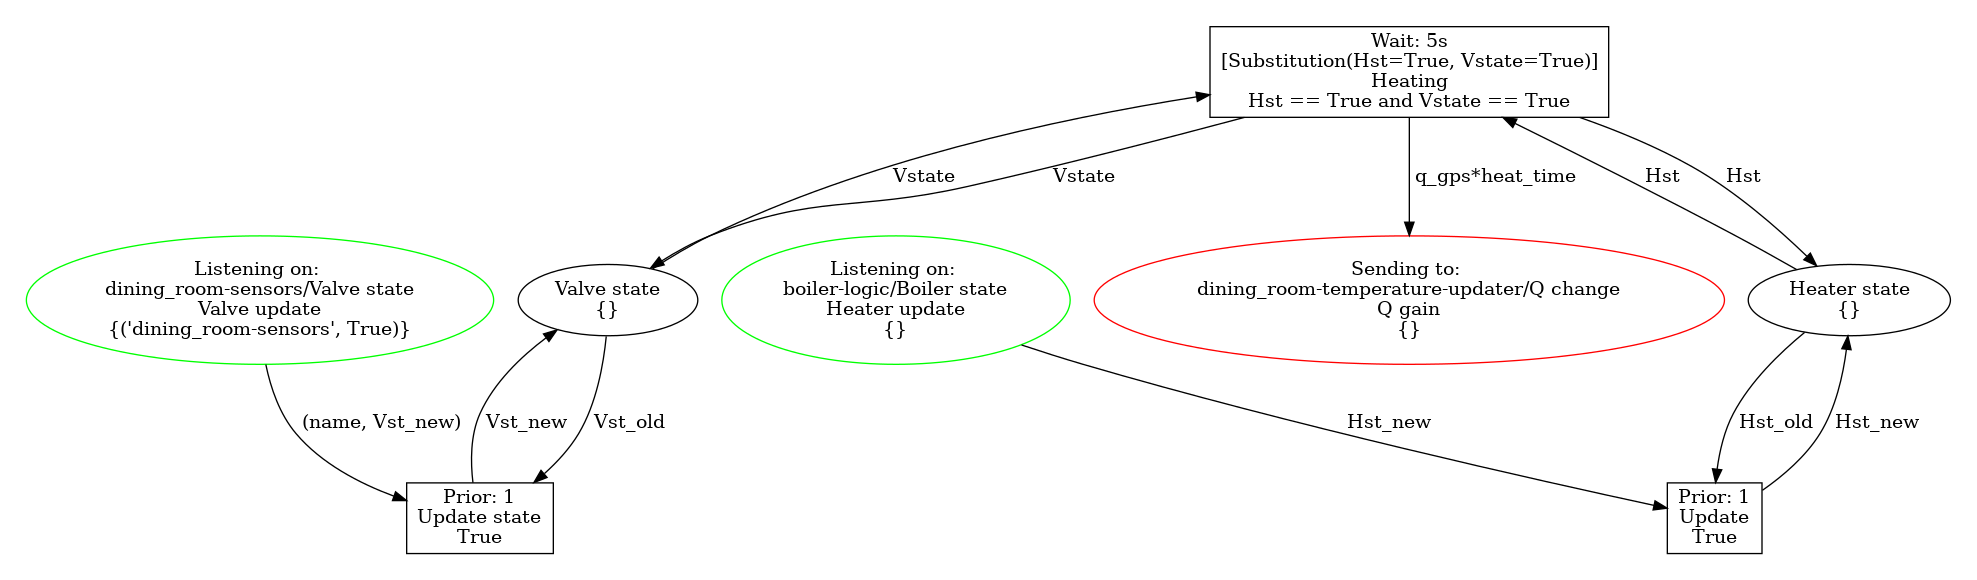
\includegraphics[width=\textwidth]{obrazky-figures/room-heating.png}
 \caption{Simulace ohřívání pokojů.}
 \label{heater-viz}
\end{figure}

\begin{figure}[htb]
 \centering
 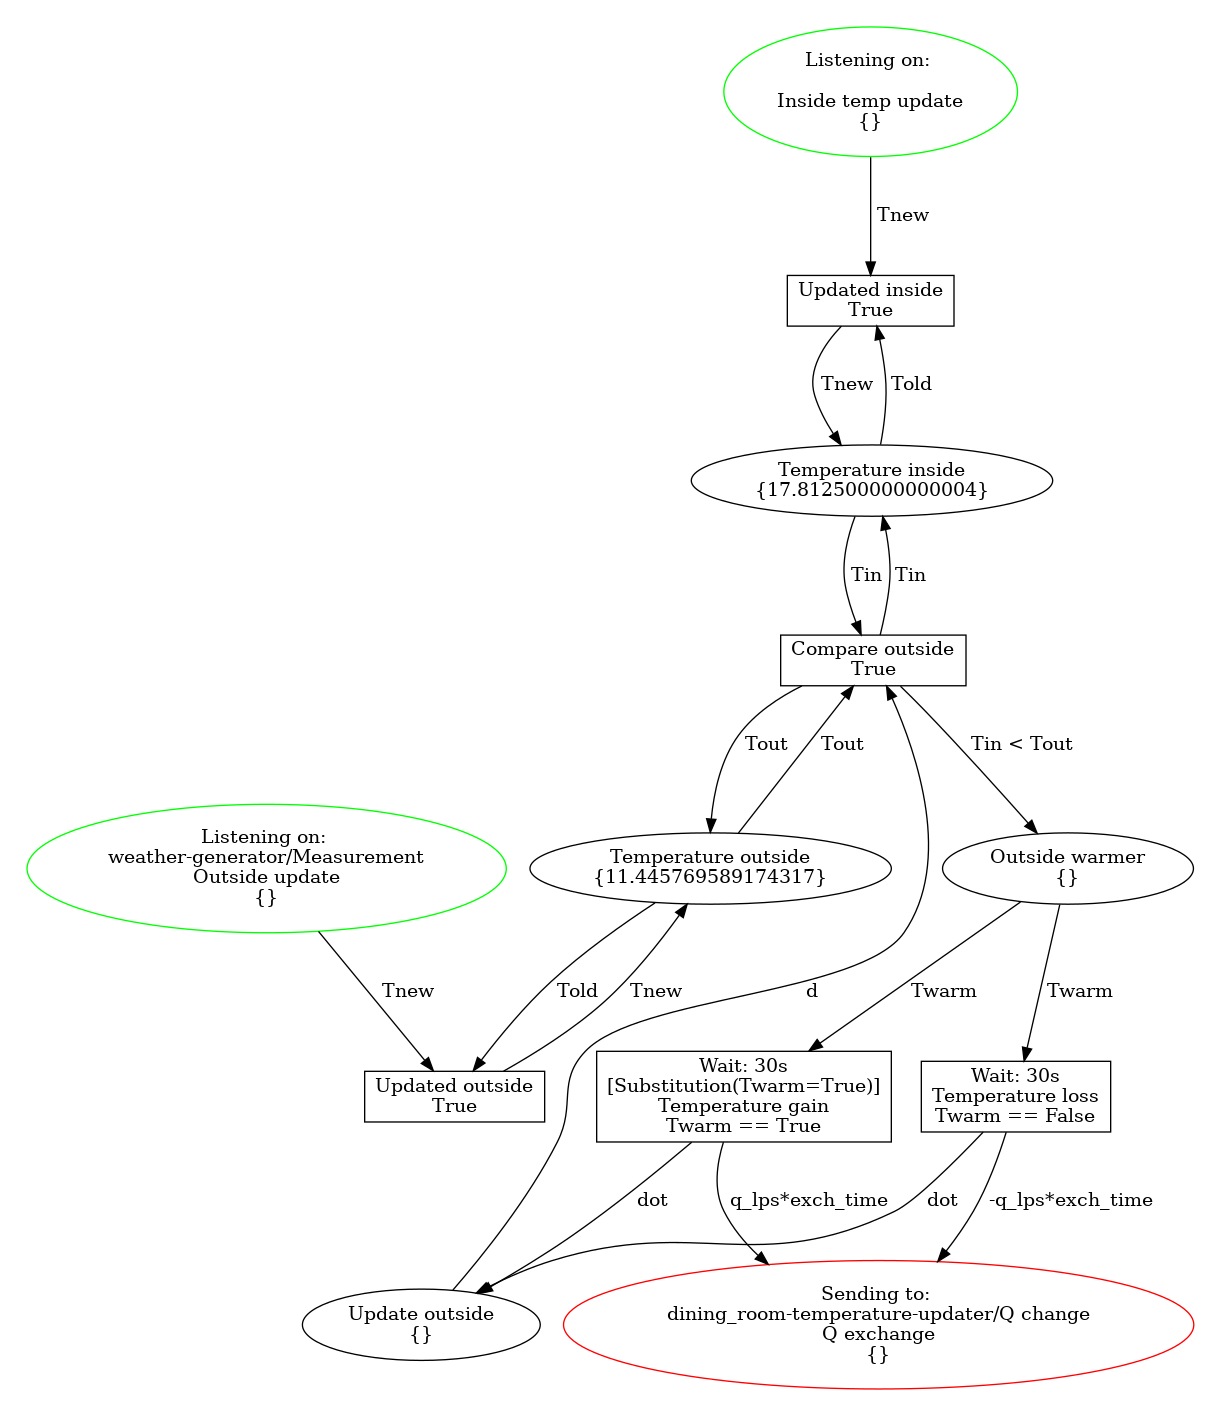
\includegraphics[width=\textwidth]{obrazky-figures/room-exchange.png}
 \caption{Simulace výměny teploty se vnějším prostředím.}
 \label{exchange-viz}
\end{figure}


\section{Řízení pokojů}
\label{sec:server-details}

Následující Petriho sítě provádějí obsluhu systému pokojů. K~nim patří, například řízení senzoru \ref{subsec:room-control} a tabulka očekávaných teplot v~pokoji \ref{subsec:room-table} během dané hodiny.

\subsection{Řízení}
\label{subsec:room-control}

Řízení pokojů je vizualizované na obrázku \ref{sensor-viz}. Funkce senzoru je velice jednoduchá, a spočívá v~oznámení bojleru že pokoj potřebuje zapnout ohřívaní. To se provádí odesíláním dvojici \uv{\texttt{("jméno pokoje", "ventil je otevřen")}} z~portu \uv{\texttt{Valve state}}. Pro splnění tohoto úkolu, síť potřebuje porovnat hodnoty očekávané teploty pro daný pokoj na tento čas, a současné teploty v~pokoji. Informací o~poslední přichází do portu \uv{\texttt{Temperature inside}}. Takové srovnání se musí provádět jen tehdy, kdy se stane nějaká změna v~současné teplotě pokoje.  Pro oznámení změn teploty uvnitř, slouží port \uv{\texttt{Temperature update}}. Současný stav očekávané teploty se ukládá do místa \uv{\texttt{Expected temperature}}.

\subsection{Tabulka očekávaných teplot}
\label{subsec:room-table}

Účelem této Petrího sítí je dynamická změna očekávané teploty v~pokoji podle příchozí hodnoty času. Tu, Petriho síť na obrázku \ref{room-table-viz} obdrží ze vstupního portu pod názvem \uv{\texttt{Time update}}. Následující obsah tabulky je vytvořen dynamicky. Jsou to místa pod názvem Time-HH:MM, obsahující číselný token, reprezentující  počet vteřin z~počátku dne. Té hodnoty se použijí pro zjišťování, do kterého časového rozmezí spadá nová hodnota času. Podle něj určí teplota v~pokoji por danou dobu, která se vezme z~výstupní šipky přechodu s~názvy \uv{\texttt{Enable: HH:MM--HH:MM}}. Výsledek bude uložen do místa \uv{\texttt{Expected update}}.

Pokud nová hodnota očekávané teploty se liší od předchozí, která je uložena v~místě \uv{\texttt{Expected temperature}}, tak ta změna bude předaná pro odesílaní výstupnímu portu \uv{\texttt{Temperature update}}.

\begin{figure}[htb]
 \centering
 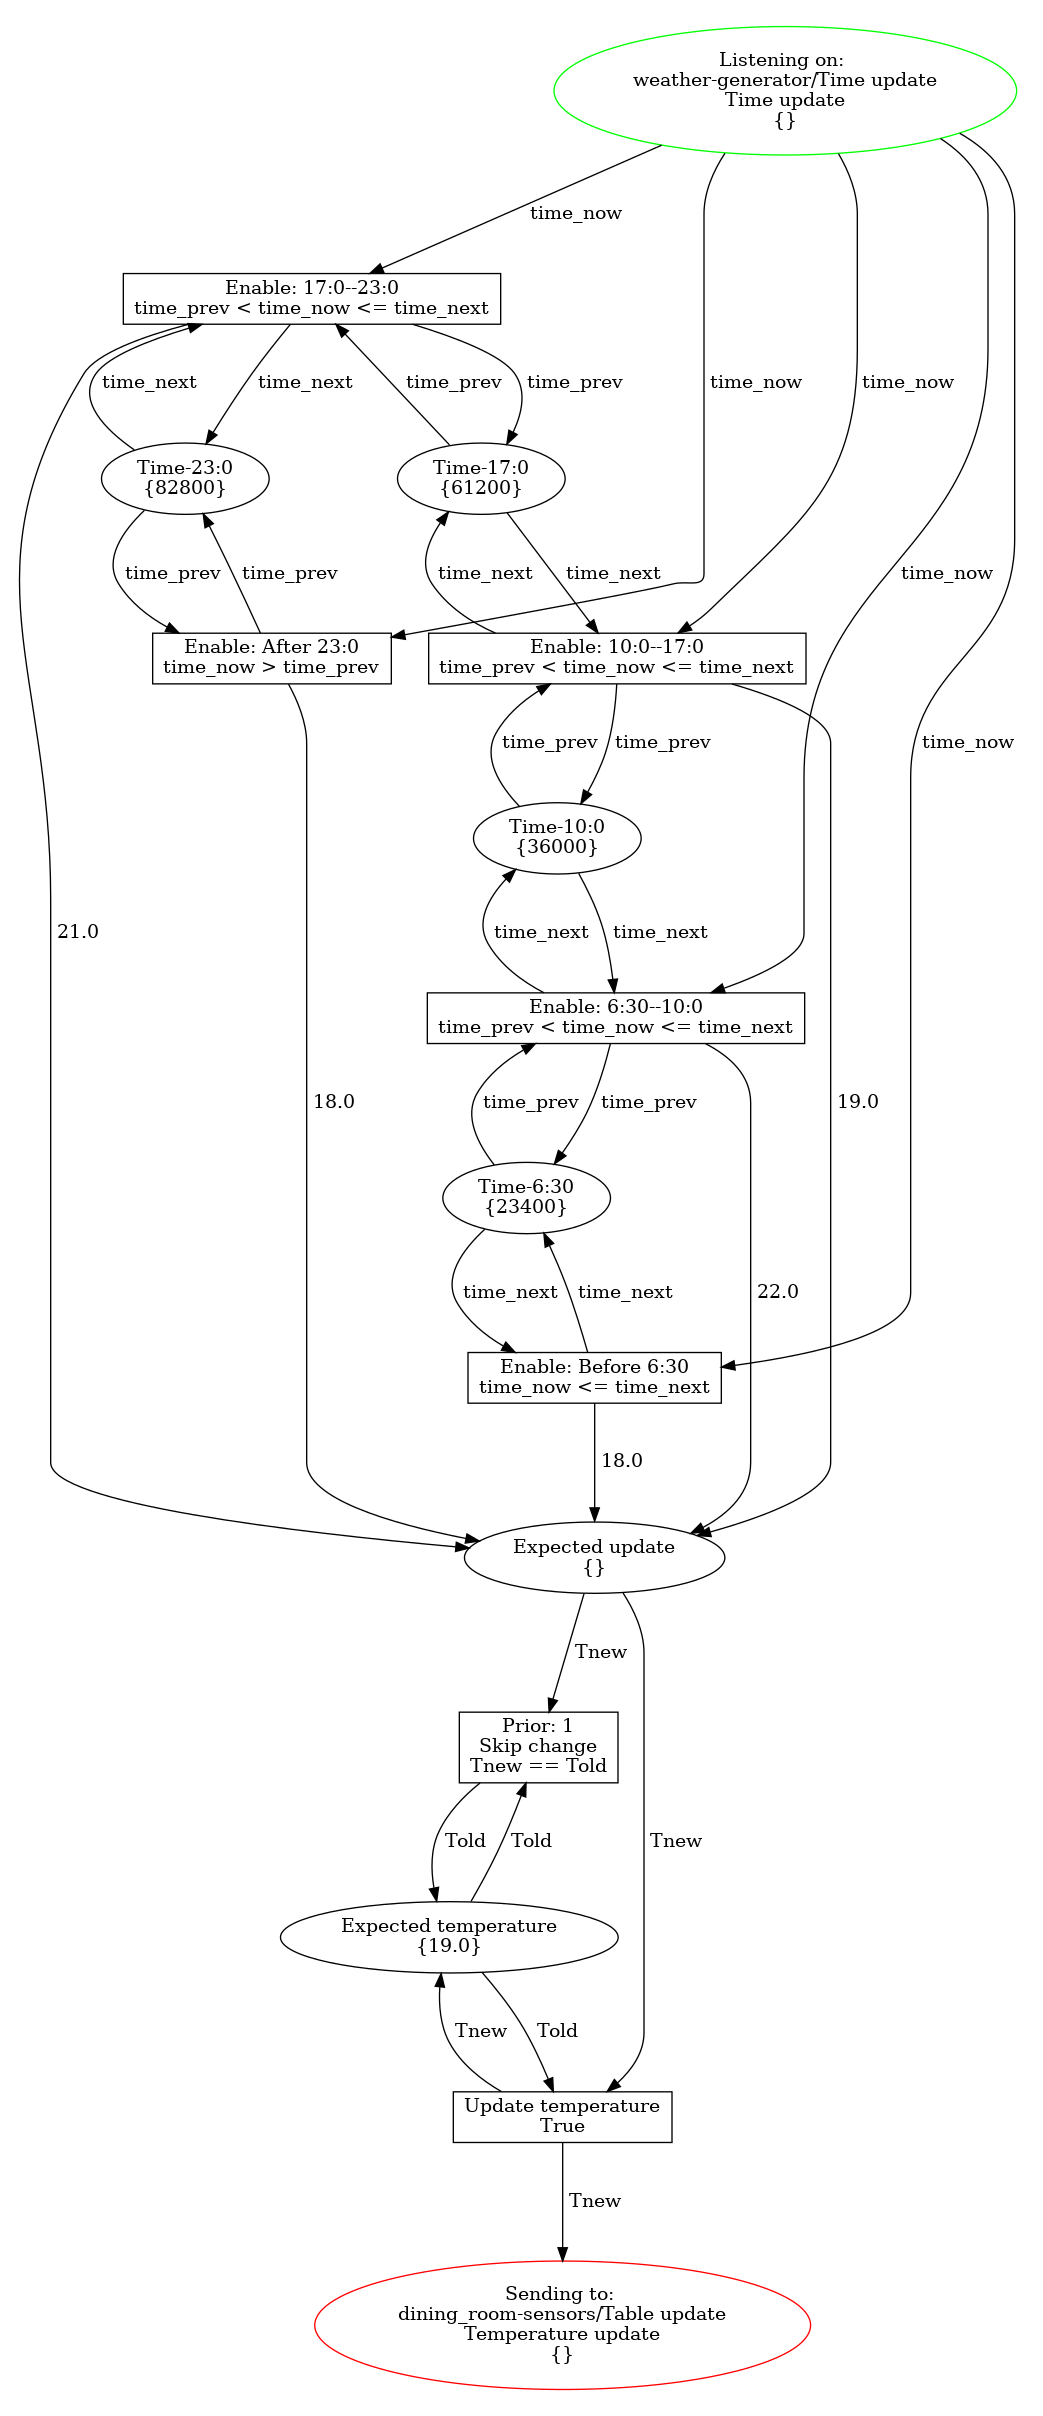
\includegraphics[width=0.6\textwidth]{obrazky-figures/room-timetable.png}
 \caption{Tabulka teplot pro pokoj.}
 \label{room-table-viz}
\end{figure}

\begin{figure}[htb]
 \centering
 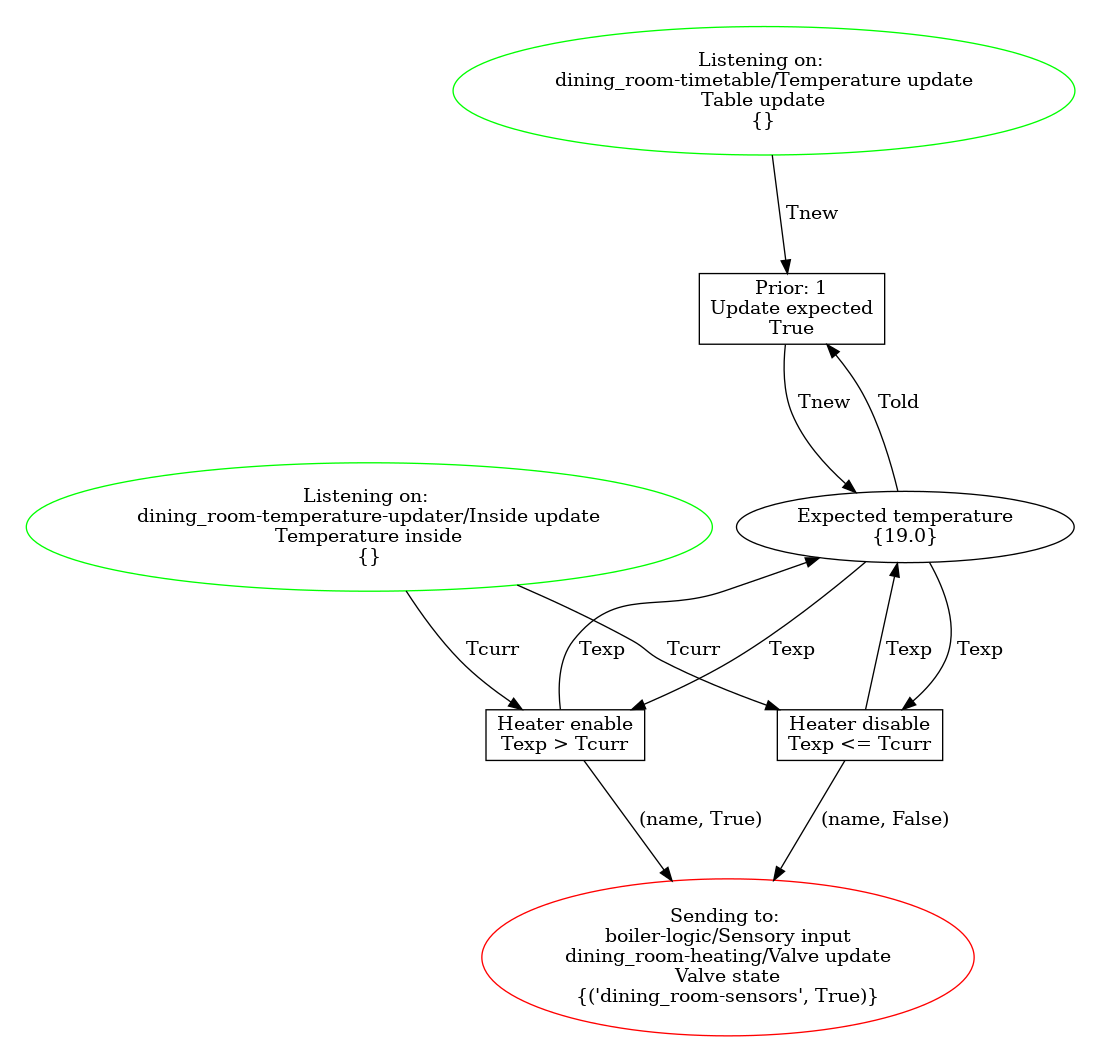
\includegraphics[width=\textwidth]{obrazky-figures/room-sensors.png}
 \caption{Simulace senzorů a stavu ventilů v~pokoji.}
 \label{sensor-viz}
\end{figure}


\section{Simulace bojleru}
\label{sec:boiler-net-details}

Součásti simulace je taky popis chování bojleru. Jeho cílem je sledování stavu ventilů v~pokojích. Sémantika je jednoduchá -- pokud je nějaký z~pokojů má otevřený ventil, on to oznámí vstupnímu portu \uv{\texttt{Sensory input}} dvojicí tokenů \texttt{("name", "enabled")}. Když alespoň jeden pokoj má otevřený ventil, tak bojler musí začít pracovat na jeho ohřáti.

Celá síť obsahuje dvá základní řídící místa -- \uv{\texttt{Table}} a \uv{\texttt{Active Table}}. První je tabulka registrace pokojů. Tam se ukládá aktuální stav ventilu pokoje, dokud nebyla změna jeho stavu zpracovaná aktivní tabulkou. V~aktivní tabulce se nacházejí pokoje, které v~danou chvílí požadují zapnuté topení. Pokud je v~ní alespoň jeden takový pokoj, tak bojler se přepne do zapnutého stavu. Současný stav bojleru je uložen v~místě \uv{\texttt{Boiler Enabled}}, a změny jeho stavu se oznamují na výstupní port \uv{\texttt{Boiler state}}.

Výsledná síť je na na obrázku \ref{boiler-logic-viz}.

\begin{figure}[httb]
 \centering
 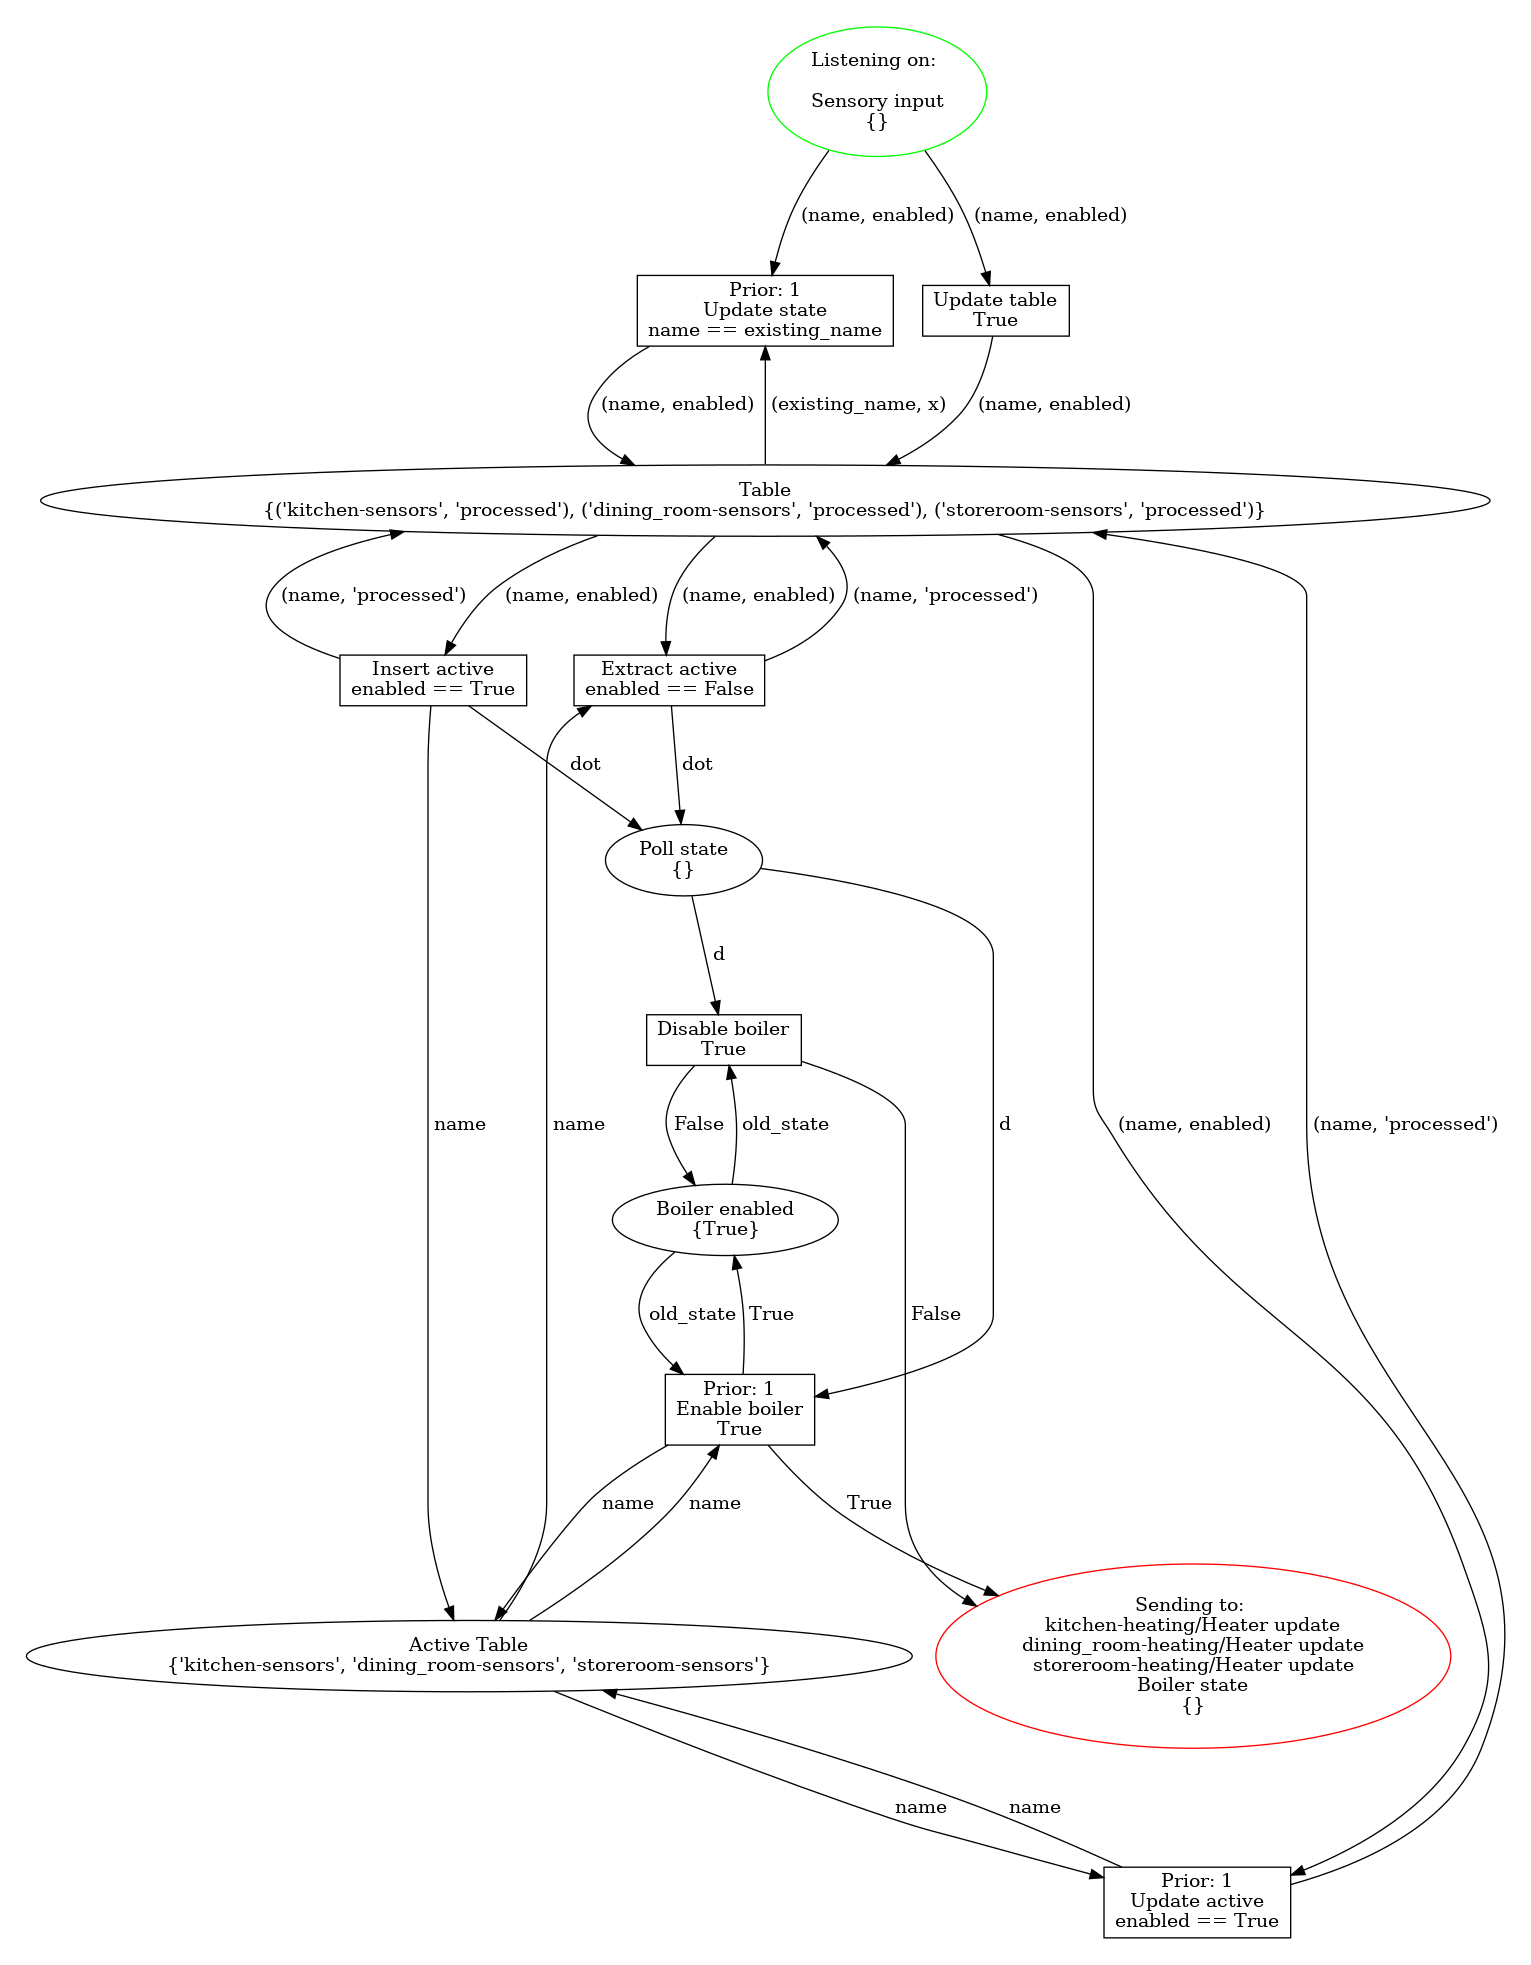
\includegraphics[width=\textwidth]{obrazky-figures/boiler-logic.png}
 \caption{Simulace bojleru.}
 \label{boiler-logic-viz}
\end{figure}

\section{Nahrazení simulace realitou}

Stojí za to se zmínit, že účelem této aplikace není zcela přesná simulace chování topení, ale její zjednodušená kopie. Do úvahy se nebere například to, že rychlost výměny tepla s~vnějším prostředím není konstantní, jak je uvedeno v~tabulce \ref{tab:tepelne-ztraty}, ale je závislá na spoustě parametrů, jako teplota vnějšího prostředí, materiál a tloušťka stěn pokoje atd. To se nepočítá v~současném návrhu, ale může být přidáno ve případě potřeby. Účelem této aplikace je vizualizace práce vytvořeného simulátoru a demonstrace využití v~distribuovaných systémech.

Každou Petriho síť z~popsané aplikace by bylo možné vyměnit za reální součástku, zcela nebo částečně. Ve případě že by uživatel měl už existující system topení, ale by chtěl odzkoušet nová čidla pro měření teploty v~pokoji, a jejich řízení, tak by se dalo popsat chování čidel Petriho sítí, a provázat síť vstupními a výstupními porty s~už existujícími součástkami. Požaduje se od tech součástek jenom podpora MQTT a dodržení zásad vložení externí aplikace z~podsekci \ref{subsec:comm-proto}.

\chapter{Detailní popis implementace Petriho sítě v~rámci simulátoru.}
\label{chap:postup}

V~této kapitole je detailní popis vytvoření Petriho sítě, simulující chování počasí během dne \ref{weather-viz}.

\section{Měření teploty venku}
\label{sec:mereni-teploty}
Modelování chování teploty venku je stochasticky proces, který není možné spočítat přesně. Ale ve snaze její simulace byla navržena Petriho síť, využívající pravděpodobnostní přechody. Má na vstupu rozsah teplot den -- noc a podle vybrané doby dne, za použití funkce $cos$ modeluje změnu aktuální teploty. Rozhodnutí použití funkce $cos$ vychází z~jednoduchého pozorování průběhu teplot během dne a periodicita změny teploty se jí trochu \href{https://forecast.weather.gov/MapClick.php?lat=42.3758&lon=-71.1187&lg=english&FcstType=graphical}{podobá} za předpokladu, že průběh funkce začíná v~nejteplejší hodinu během dne, což je počáteční bod funkce $cos$. Ale základní cíl použité funkce je modelování spojitého průběh teplotních změn.

Pravděpodobnostní přechody modelují náhodné jevy jako oteplení nebo ochlazení kvůli východu slunce a jiné. Ukázku implementace můžete vidět v~\ref{prob-ev-viz}.

Vizuální reprezentací celé sítě můžete vidět na obrázku \ref{weather-viz}.

Obrázek \ref{weather-viz} byl vygenerován v~průběhu práci simulátoru, díky použítí rozšíření \href{https://www.ibisc.univ-evry.fr/~fpommereau/SNAKES/API/plugins/gv.html}{\uv{gv}}. Toto rozšíření, spolu s~menšími vizuálními změnami jiných rozšíření, zaměřených na jednotlivé prvky sítě, dokáže spolehlivě vygenerovat obrázek Petriho sítě, podobný \ref{weather-viz}, v~jakýkoliv okamžik simulace. Pro vytvoření obrázku je specifikován jednoduchý příkaz \pyth{draw("file.png")}.


Tato síť je poměrně jednoduchá na pochopení, a zároveň názorně ukazuje použítí většiny naimplementovaných rozšíření. Celý postup pro vytvoření \ref{weather-viz} se sestavuje z~následujících kroků -- \ref{sec:process-steps}.

\section{Kroky postupů}
\label{sec:process-steps}

\paragraph{Krok 1:}

Je důležité si nejdříve naimportovat rozšíření a knihovnu SNAKES podle \ref{code:plugin-setup}. Každá síť si vytváří klauzuli \pyth{PetriNet('nazev site')}. Dále se do sítě musí přidat místa, přechody, a případně vstupní a výstupní porty, při použití nastavení podle \ref{subsec:remote-ports-setup}.

V~případě potřeby se dá vytvořená síť vykreslit pomocí příkazu \pyth{draw(net_name+'.png')}

\begin{python}
 # Import pluginu, knihovny SNAKES, viz (*\ref{code:plugin-setup}*) (*\label{code:thermometr-draw}*)
 net_name="Thermometr"
 n=PetriNet(net_name)
 (*\ldots*) # Specifikace prechodu a mist: (*\ref{therm-gen-viz}*), (*\ref{therm-calc-viz}*) a (*\ref{prob-ev-viz}*)
 n.draw(f"{path_to_img}/{net_name}.png")
\end{python}

\paragraph{Krok 2:}

Dále, abychom si namodelovali chování teploty během dne, musíme vytvořit generátor, který rozdělí den častí. V~případě této implementace je to $48$ -- \ref{code:poll-freq}. Tedy každých $1800s$ se vytvoří nová teplota -- \ref{code:timed-temp-example}, což je použití rozšíření \texttt{timed\_pl} z~\ref{subsec:timed_pl}. Výsledek je na obrázku \ref{therm-gen-viz}.

\begin{python}
 # Sit (*\ref{therm-gen-viz}*) (*\label{code:gen-therm-draw}*)
 f=48 # Frekvence mereni behem dne (*\label{code:poll-freq}*)
 T=24*60*60/f # Perioda zmen teploty
 k=0 # Citac pro generator
 timeout=T
  # Deklarace globalnich promenych v~ramci site
 n.declare(f"f={f}") (*\label{code:snakes-glob-var}*)
  # Vytvoreni mist
 gen=Place("Generator", [k], check=tInteger)
 gen_k=Place("Generator_k", [], check=tInteger)
 # Pridani mist do site
 n.add_place(gen)
 n.add_place(gen_k)

 # Vytvoreni prechodu
 takt=Transition("takt", timeout=timeout) (*\label{code:timed-temp-example}*)
 takt.add_input(gen, Variable("k"))
 takt.add_output(gen, Expression("(1 + k) % f"))
 takt.add_output(gen_k, Variable("k"))
 # A~pridani do site
 n.add_transition(takt)
\end{python}

\begin{figure}[htb]
 \centering
 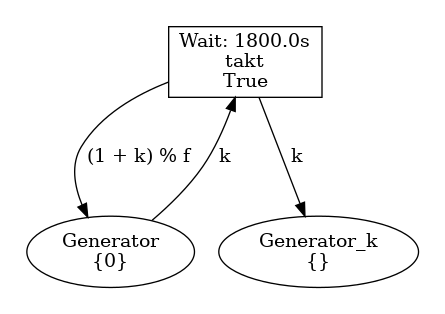
\includegraphics[width=0.4\textwidth]{obrazky-figures/therm-gen.png}
 \caption{Generator doby dne.}
 \label{therm-gen-viz}
\end{figure}

\paragraph{Krok 3:}
Pro vytvoření teploty pro daný okamžik musíme provést mapování na teplotní funkci \ref{code:decl-func}. To se provádí na výstupu z~\pyth{Transition("tcalc")}, a je povolené podle pravidel \href{https://www.ibisc.univ-evry.fr/~fpommereau/SNAKES/understanding-transition-firing.html}{anotaci} výstupních šípek. Funkce vrací číselnou hodnotu v~rozmezí $5-18\left[C^{\circ}\right]$, která se vloží do místa \pyth{Place("Temp_placement", [(low, high)], check=tTuple)} z~\ref{code:temp_pl}.

Výsledná síť je na obrázku \ref{therm-calc-viz}.

\begin{python}
 # Sit (*\ref{therm-calc-viz}*)
 # Globalni promene (*\label{code:therm-calc-draw}*)
 low, high=5, 18
 # Deklarace globalni knihovny a funkce pro vypocet teploty
 n.declare("from math import cos, pi") (*\label{code:decl-libs}*)
 n.declare("def temp_placement(Tmin, Tmax, k):" (*\label{code:decl-func}*)
 "\n\tif k~== 0:"
 "\n\t\treturn float(format(Tmax, \".1f\"))"
 "\n\telse:"
 "\n\t\treturn float(format("
 "Tmin + (Tmax-Tmin)*(cos(2*pi*k/f)/2 + 1/2)," (*\label{code:lib-import-usage}*)
 "\".1f\"))")

 # Vytvoreni mist
 temp_pl=Place("Temp_placement", [(low, high)], check=tTuple) (*\label{code:temp_pl}*)
 traw=Place("Temperature_raw", [], check=tFloat)
 n.add_place(temp_pl)
 n.add_place(traw)

 # Pridani prechodu
 tcalc=Transition("tcalc")
 tcalc.add_input(gen_k, Variable("k"))
 tcalc.add_output(traw, Expression("temp_placement(Tmin, Tmax, k)"))
 tcalc.add_input(temp_pl, Tuple((
   Variable("Tmin"), Variable("Tmax"))))
 tcalc.add_output(temp_pl, Tuple((
   Variable("Tmin"), Variable("Tmax"))))
 n.add_transition(tcalc)
\end{python}

\begin{figure}[htb]
 \centering
 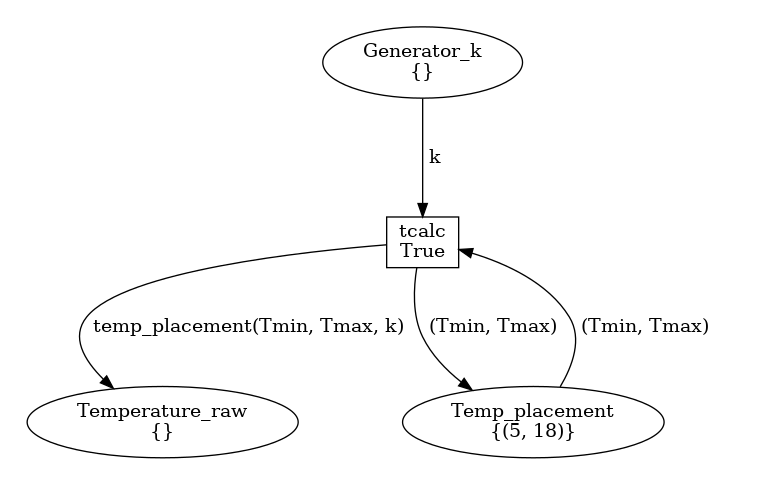
\includegraphics[width=0.6\textwidth]{obrazky-figures/calc.png}
 \caption{Výpočet teploty pro danou dobu dne.}
 \label{therm-calc-viz}
\end{figure}

\paragraph{Krok 4:}

Tato síť je zaměřena na simulaci počasí z~pohledu zdí budovy, která se čelí vnějšímu prostředí. Simulace je v~tomto případě hrubou, ale dostačující aproximaci reálného světa.

Pro simulaci různých náhodných jevů slouží \ref{code:prob-ev-draw}. Pro případ, že teplota přesně odpovídá očekávané, je přechod \pyth{texpec=Transition("texpec", prob=0.6)} z~\ref{code:texpec}. Ten má pravděpodobnost $0.6$. Pak jsou stejné pravděpodobnosti $0.2$ pro případ deště nebo slunce, které svítí na zeď a jsou to řádky \ref{code:tsunny} a \ref{code:texpec}. Součet pravděpodobnosti musí být vždy $1$. Pro seskupení takových přechodů slouží řádek \ref{code:prob-temp-neghb-example-1} a \ref{code:prob-temp-neghb-example-2}. Přechody musí mít stejnou sadu vstupních míst, jak je to popsané v~\ref{subsec:prob_pl}.

Síť vypadá následovně: \ref{prob-ev-viz}.

\begin{python}
 # Sit (*\ref{prob-ev-viz}*)
 # Import globalnich knihoven (*\label{code:prob-ev-draw}*)
 n.declare("from random import random")

 # Pridani vystupnich mist
 meas=Place("Measurement", [0.], check=tFloat)
 n.add_place(meas)

 # Nastaveni mista jako vystupni port
 n.add_remote_output(meas, "temp_sens/Input temp")

 trainy=Transition("trainy", prob=0.2) (*\label{code:prob-temp-example}*) (*\label{code:trainy}*)
 tsunny=Transition("tsunny", prob=0.2) (*\label{code:tsunny}*)
 texpec=Transition("texpec", prob=0.6) (*\label{code:texpec}*)
 # Spojeni prechodu do skupiny
 trainy.add_neighbour_transition(texpec) (*\label{code:prob-temp-neghb-example-1}*)
 trainy.add_neighbour_transition(tsunny) (*\label{code:prob-temp-neghb-example-2}*)

 # Nahodna zmena teploty vedouci k~ochlazeni
 trainy.add_input(traw, Variable("Tnew"))
 trainy.add_output(meas, Expression("Tnew-random()*2"))
 n.add_transition(trainy)

 # Teplota podle ocekavani
 tsunny.add_input(traw, Variable("Tnew"))
 tsunny.add_output(meas, Expression("Tnew+random()*2"))
 n.add_transition(tsunny)

 # Zvyseni teploty na porovnani s~ocekavanou
 texpec.add_input(traw, Variable("Tnew"))
 texpec.add_output(meas, Variable("Tnew"))
 n.add_transition(texpec)
\end{python}

\begin{figure}[htb]
 \centering
 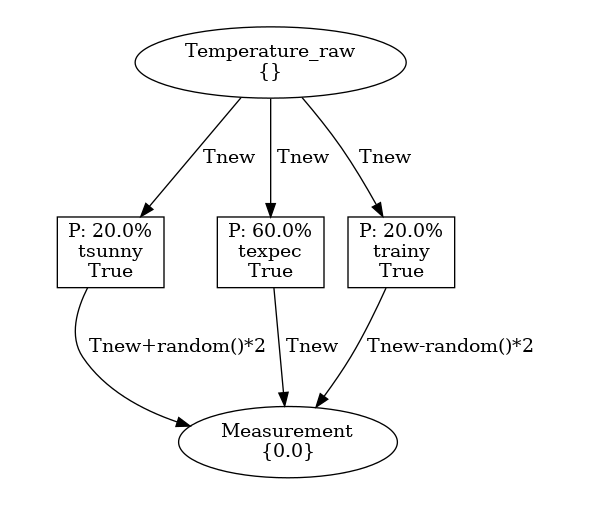
\includegraphics[width=0.6\textwidth]{obrazky-figures/measure.png}
 \caption{Modelování náhodných změn teplot.}
 \label{prob-ev-viz}
\end{figure}

\chapter{Závěr}
\label{chap:zaver}

Během čtení této bakalářské práce byla čtenářovi nabídnuta možnost pochopit teoretické základy Petriho sítí, zjistit rozdíl mezí značkovanými a vysokoúrovňovými Petriho sítěmi a nahlédnout do případů, kde se tento modelovací prostředek úspěšně používá nebo má předpoklady pro uplatnění. Byly taky ukázaný teoretické základy Grafů Vysokoúrovňových Petriho sítí, které našli využití v~dalších kapitolách, spojených s~vizualizací navržené aplikace simulatoru.

Byla vyjasněna problematika Distribuovaných systémů, a taky kde a proč se takové systémy používají. Byl vysvětlen pojem Diskrétní simulace a simulace v~reálném čase, včetně jejich běžných případů využití v~praxi. V~sekci spojené s~teoretickými základy simulátoru bylo taky řečeno o~jeho využití v~HWIL. Ve stejné sekci byl podrobně popsán MQTT protokol komunikace, který našel svoje využití v~mnoha místech, včetně implementací simulátoru.

Další kapitola vyjasnila struktura simulatoru, využívající MQTT protokol. Značná část této kapitoly byla zaměřená na vysvětlení práce vlastního protokolu pro nastavení a využití simulátoru, který se dá uplatnit pro napsaní externích aplikací pro výsledný simulátor. Stejně tak zde byla velice podrobně popsána implementace několika rozšíření pro knihovnu SNAKES, bez kterých využití simulačního nástroje není možné. Z~toho důvodu byl zdůrazněn postup pro import těchto rozšíření do knihovny SNAKES.

Stejně jako bez rozšíření, simulátor Petriho sítí v~reálném čase by nebyl možný bez implementace plánovače událostí, informace, která byla popsána v~další sekci.

Následující kapitola měla za úkol vyjasnit návrh aplikace, demonstrující využití simulátoru pro modelování a simulaci distribuovaných systémů na příkladě chování tepelného řízení. Spolu s~kapitolou \ref{chap:app-implementation} se zcela podrobně popsala práce navržené aplikace.

Poslední kapitolou této práce byla ukázka implementaci jedné z~Petriho sítí, patřící do aplikace, která demonstrovala využití všech navržených rozšíření a měla za účel naučit uživatele správně zacházet s~knihovnou SNAKES, a tedy implementovat svoje vlastní nápady. Pro tento účel slouží appendix \ref{chap:instal-tutor}, který obsahuje instalační manuál a popisuje nástroje, usnadňující nastavení simulátoru do 2 řádku kódu.

Svoji práci tímto ukončuji a považuji za zcela hotovou. Byly splněny všechny body zadání, naimplementované a otestované všechny nástroje a dodrženy všechny pravidla strukturování textu, patřící technické zprávě, podle standardů VUT.





  
  % Kompilace po částech (viz výše, nutno odkomentovat)
  % Compilation piecewise (see above, it is necessary to uncomment it)
  %\subfile{projekt-01-uvod-introduction}
  % ...
  %\subfile{chapters/projekt-05-conclusion}


  % Pouzita literatura / Bibliography
  % ----------------------------------------------
\ifslovak
  \makeatletter
  \def\@openbib@code{\addcontentsline{toc}{chapter}{Literatúra}}
  \makeatother
  \bibliographystyle{bib-styles/slovakiso}
\else
  \ifczech
    \makeatletter
    \def\@openbib@code{\addcontentsline{toc}{chapter}{Literatura}}
    \makeatother
    \bibliographystyle{bib-styles/czechiso}
  \else 
    \makeatletter
    \def\@openbib@code{\addcontentsline{toc}{chapter}{Bibliography}}
    \makeatother
    \bibliographystyle{bib-styles/englishiso}
  %  \bibliographystyle{alpha}
  \fi
\fi
  \begin{flushleft}
  \bibliography{projekt-20-literatura-bibliography}
  \end{flushleft}

  % vynechani stranky v oboustrannem rezimu
  % Skip the page in the two-sided mode
  \iftwoside
    \cleardoublepage
  \fi

  % Prilohy / Appendices
  % ---------------------------------------------
  \appendix
\ifczech
  \renewcommand{\appendixpagename}{Přílohy}
  \renewcommand{\appendixtocname}{Přílohy}
  \renewcommand{\appendixname}{Příloha}
\fi
\ifslovak
  \renewcommand{\appendixpagename}{Prílohy}
  \renewcommand{\appendixtocname}{Prílohy}
  \renewcommand{\appendixname}{Príloha}
\fi
%  \appendixpage

% vynechani stranky v oboustrannem rezimu
% Skip the page in the two-sided mode
%\iftwoside
%  \cleardoublepage
%\fi
  
\ifslovak
%  \section*{Zoznam príloh}
%  \addcontentsline{toc}{section}{Zoznam príloh}
\else
  \ifczech
%    \section*{Seznam příloh}
%    \addcontentsline{toc}{section}{Seznam příloh}
  \else
%    \section*{List of Appendices}
%    \addcontentsline{toc}{section}{List of Appendices}
  \fi
\fi
  \startcontents[chapters]
  \setlength{\parskip}{0pt}
  % seznam příloh / list of appendices
  % \printcontents[chapters]{l}{0}{\setcounter{tocdepth}{2}}
  
  \ifODSAZ
    \setlength{\parskip}{0.5\bigskipamount}
  \else
    \setlength{\parskip}{0pt}
  \fi
  
  % vynechani stranky v oboustrannem rezimu
  \iftwoside
    \cleardoublepage
  \fi
  
  % Přílohy / Appendices
  % Tento soubor nahraďte vlastním souborem s přílohami (nadpisy níže jsou pouze pro příklad)
% This file should be replaced with your file with an appendices (headings below are examples only)

% Umístění obsahu paměťového média do příloh je vhodné konzultovat s vedoucím
% Placing of table of contents of the memory media here should be consulted with a supervisor
%\chapter{Obsah přiloženého paměťového média}

\chapter{Instalační manuál}

Pokud byste potřebovali odzkoušet simulační nástroj z této práci, tak bych doporučoval udělat této kroky instalace.
\begin{enumerate}
    \item Nainstalovat si balíčky \texttt{python3.6}, \texttt{graphviz}, \texttt{python3-pip}, \texttt{git}.
    \item Nainstalovat knihovnu SNAKES podle nějakého z postupu v \href{https://www.ibisc.univ-evry.fr/~fpommereau/SNAKES/first-steps-with-snakes.html}{návodu}. \label{pip-snakes}
    Doporučený postup, nainstalovat to přes pip:

    \texttt{pip3 install git+git://github.com/fpom/snakes \-\-user}.
    \item Nainstalovat této knihovny přes \texttt{pip3 install xxx \-\-user} pro podporu MQTT, kde \texttt{xxx} je:
    \begin{itemize}
        \item \texttt{pahomqtt}
        \item \texttt{hbmqtt}
    \end{itemize}
    \item Naklonovat git repositář simulační knihovny do libovolného místa na disku:

    \href{https://github.com/Danil-Grigorev/rt-sim-petry-net}{\texttt{https://github.com/Danil-Grigorev/rt-sim-petry-net}}.
    \item Provést potřebné úpravy pro rozšíření \uv{gv} v poslední verzí knihovny SNAKES, a nakopírovat jiné rozšíření do složky pro rozšíření. Tá se obecně po kroku \ref{pip-snakes} nachází v \texttt{$\sim$/.local/lib/python3.6/site-packages/snakes/plugins}, ale může se to lišit v závislosti od nastavení balíčku Python. Seznám rozšíření pro kopírovaní/nahrazení ze složky \texttt{rt-sim-petry-net/plugins} je následující:
    \begin{itemize}
        \item \texttt{prior\_pl.py}
        \item \texttt{prob\_pl.py}
        \item \texttt{sim\_pl.py}
        \item \texttt{timed\_pl.py}
        \item \texttt{gv.py}
    \end{itemize}

\end{enumerate}

  
  % Kompilace po částech (viz výše, nutno odkomentovat)
  % Compilation piecewise (see above, it is necessary to uncomment it)
  %\subfile{projekt-30-prilohy-appendices}
  
\end{document}
